\documentclass{article}
\usepackage[utf8]{inputenc}
\usepackage[spanish]{babel}
\usepackage[hidelinks]{hyperref}
\usepackage{setspace}
\usepackage{graphicx}
\usepackage{float}
\usepackage[hidelinks]{hyperref}
\usepackage{dirtree}
\usepackage{pdflscape}
\usepackage{pdfpages}


\usepackage[compact]{titlesec}
\usepackage{geometry}
\geometry{
   a4paper,
   total={170mm,257mm},
   left=30mm, % entre 25-35
   right=30mm, % entre 25-35
   top=30mm, % no más de 30
   bottom=25mm, % no más de 30
}

\usepackage{fancyhdr}
\pagestyle{fancy}
\fancyhf{}
\lhead{}
\rhead{Bárbaros Software S.A.}
\rfoot{\thepage}
\lfoot{Plan de gestión, análisis, diseño y memorial del proyecto KeyPaX}
\renewcommand{\footrulewidth}{0.4pt}

\setlength{\parindent}{2em}
\setlength{\parskip}{1em}

\begin{document}

\begin{titlepage}
   \centering
   \vspace*{\fill}

   \vspace*{0.5cm}

   \Huge
   \textbf{Plan de gestión, análisis, diseño y memorial del proyecto KeyPaX}

   \vspace*{0.5cm}

   \huge
   Bárbaros Software S.A. (Grupo 3)

   
\includegraphics[height=5cm,angle=-45]{../images/llave.png}

   \begin{Large}
       Carlos Bellvis, 755452\\
       Jorge Bernal, 775695\\
       Jorge Borque, 777959\\
       Arturo Calvera, 776303\\
       Andoni Salcedo, 785649\\
       Javier Vela, 775593\\
   \end{Large}

   \vspace*{1cm}

   \large
   \href{https://github.com/UNIZAR-30226-2021-03}{Organización GitHub: https://github.com/UNIZAR-30226-2021-03}

   \vspace*{\fill}

\end{titlepage}

\pagebreak

\tableofcontents

\pagebreak

\section{Introducción}

En el siguiente documento se presenta el sistema KeyPaX, va a ser desarrollado por Bárbaros Software S.A. y permite gestionar contraseñas almacenadas remotamente en los servidores del sistema. Permite almacenar junto con las contraseñas el nombre de usuario, URL y una descripción textual, entre otros. Las contraseñas se pueden organizar por categorías para subdividir las contraseñas por temática.

Además, para mejorar la seguridad del sistema, se podrán generar automáticamente contraseñas robustas con longitud y caracteres variables. El usuario accederá al servicio mediante una contraseña maestra y deberá identificarse en el inicio de sesión mediante el 2FA.

Para acceder al sistema se utilizará la aplicación para móviles Android o en navegador web. Se utilizará Java (Android SDK) y JavaScript (React.JS), respectivamente, para implementar las vistas del sistema. El \textit{backend} se desarrollará utilizando Node.JS y la \textit{framework} Express. Por último, la base de datos utilizará el SGBD MongoDB.

El despliegue del sistema se realizará en un entorno de contenedores Docker. Mediante Docker se puede aprovechar al máximo los recursos \textit{hardware} de la máquina, aumentando la portabilidad del sistema.

Se plantea un plan de trabajo, dónde se comprometen varias fechas para las entregas anteriores a la finalización del proyecto.  El día 15 de abril de 2021 se entregará una primera versión del sistema \textit{software}. Tras las modificaciones y correcciones propuestas por el cliente, el 21 de mayo de 2021 se presentará una segunda versión. El 1 de junio de 2021, Bárbaros Software S.A. se compromete a entregar el sistema final al cliente.

En el documento se estipulan los procesos y planes a llevar por los integrantes del proyecto al desarrollar el producto. Estos planes son precisos para llevar un análisis de calidad adecuado y para la organización de directorios del proyecto, entre otros.

Se presentan los requisitos de manera precisa y sin ambigüedades, especificando exactamente la funcionalidad del sistema. Además, se presentan varias vistas del sistema en forma de diagramas de despliegue, componentes y módulos.

Por último, se realiza una memoria del trabajo, comentando el desarrollo del proyecto y del producto. En la memoria se profundiza en la ejecución de los planes, procesos y organización propuesta, sus problemas y su resultado.

\pagebreak


\section{Organización del proyecto} \label{sec:organizacion}

El equipo del proyecto está formado por los 6 integrantes del grupo.  Para dividir el trabajo y las responsabilidades se han formado 2 grupos iniciales,  de acuerdo con las capacidades y conocimientos individuales.  Además, se ha designado como director del proyecto a Arturo Calvera, sobre el cual recae la gestión de los equipos de trabajo y de las responsabilidades de los mismos.

\begin{itemize}
   \setlength{\itemsep}{0em}
   \item \textbf{Director del proyecto}: Arturo Calvera
   \begin{itemize}
       \setlength{\itemsep}{0em}
       \item Función: Planificación y organización del equipo. Responsable de que se cumplan las tareas designadas.
   \end{itemize}
   \item \textbf{Equipo \textit{Backend}}:
   \begin{itemize}
       \setlength{\itemsep}{0em}
       \item Responsable: Arturo Calvera.
       \item Función: Desarrollo del \textit{backend} del sistema.
       \item Integrantes: Arturo Calvera, Andoni Salcedo.
   \end{itemize}
   \item \textbf{Equipo \textit{Frontend}}:
   \begin{itemize}
       \setlength{\itemsep}{0em}
       \item Responsable: Javier Vela.
       \item Sub-equipos: El equipo dedicado a la vista del sistema se divide para el desarrollo de las dos interfaces.
       \begin{itemize}
           \setlength{\itemsep}{0em}
           \item \textbf{Equipo Web}:
           \begin{itemize}
               \setlength{\itemsep}{0em}
               \item Función: Desarrollo del \textit{frontend} web del sistema.
               \item Integrantes: Jorge Bernal, Javier Vela.
           \end{itemize}
           \item \textbf{Equipo Android}:
           \begin{itemize}
               \setlength{\itemsep}{0em}
               \item Función: Desarrollo de la aplicación cliente del sistema para dispositivos Android.
               \item Integrantes: Carlos Bellvis, Jorge Borque.
           \end{itemize}
       \end{itemize}
   \end{itemize}
   \item \textbf{Aseguramiento de Calidad}: Andoni Salcedo
   \begin{itemize}
       \setlength{\itemsep}{0em}
       \item Función: Controlar el desarrollo de los planes especificados en sección \ref{sec:calidad} para el aseguramiento de la calidad del producto final.
   \end{itemize}
   \item \textbf{Transcripción de reuniones}: Javier Vela
   \begin{itemize}
       \setlength{\itemsep}{0em}
       \item Función: Registrar en actas (ficheros de texto) las decisiones y planteamientos propuestos en las reuniones del equipo. Se aplica para aquellas reuniones tanto con o sin el profesor asignado.
   \end{itemize}
   \item \textbf{Resolución de Conflictos}: Jorge Bernal
   \begin{itemize}
       \setlength{\itemsep}{0em}
       \item Función: Resolución de disputas. Actuará como mediador si surgen conflictos en cualquier ámbito del desarrollo del proyecto, pudiendo acudir a él, si se necesitase de su ayuda.
   \end{itemize}
   \item Se contempla la posibilidad de modificar dicha división en equipos para adaptarse a las necesidades que surjan durante el desarrollo del proyecto.
\end{itemize}

\pagebreak

\section{Plan de gestión del proyecto}

\subsection{Procesos}

%//////////////////////////////////////////////////////CHARLY////////////////////////////////////////////////////////
\subsubsection{Procesos de inicio}

\textbf{P.I.2} Proceso de identificación del servidor \textit{cloud} a utilizar para el despliegue.

\textbf{P.I.3} Proceso de identificación de la base de datos a utilizar.

\textbf{P.I.4} Proceso de formación inicial de cada desarrollador del equipo.

%//////////////////////////////////////////////////////BERNAL////////////////////////////////////////////////////////
\subsubsection{Procesos de ejecución y control}

\textbf{P.EC.1} Proceso de comunicación y concreción de los horarios de trabajo.

\textbf{P.EC.2} Proceso de puesta en común de trabajo realizado.

\textbf{P.EC.3} Proceso de registro de las decisiones tomadas en las reuniones.

\textbf{P.EC.4} Proceso de monitorización.
%Juntar el 2, 3 y 4 en un plan común%

\textbf{P.EC.5} Proceso de documentación del código.

\textbf{P.EC.6} Proceso de control de esfuerzos.

\textbf{P.EC.7} Proceso de entrega de resultados.

\textbf{P.EC.8} Proceso de nombrado de archivos.

%//////////////////////////////////////////////////////BORQUE////////////////////////////////////////////////////////
\textbf{P.EC.9} Proceso de estructurado de directorios.

\textbf{P.EC.10} Proceso de uso de guías de estilo.

\textbf{P.EC.11} Proceso de control de versionado y actualización del código.

\textbf{P.EC.12} Proceso de revisión del código por pares.

\textbf{P.EC.13} Proceso de revisión de los requisitos.

\textbf{P.EC.13} Proceso de ejecución de pruebas sobre el sistema.

%//////////////////////////////////////////////////////TODOS////////////////////////////////////////////////////////
\subsubsection{Procesos técnicos}

\textbf{P.T.1} Proceso de desarrollo del cliente móvil para dispositivos android implementado en Java (Android SDK).

\textbf{P.T.2} Proceso de desarrollo del \textit{frontend} web implementado en JavaScript (React.JS).

\textbf{P.T.3} Proceso de configuración de una base de datos sobre el SGBD escogido.

\textbf{P.T.4} Proceso de desarrollo del \textit{backend} utilizando Node.JS y el \textit{framework} Express.

\textbf{P.T.5} Proceso de construcción y despliegue continuo del sistema en entorno de contenedores Docker desplegado sobre máquinas virtuales en \textit{cloud}.

\pagebreak
\subsection{Planes}

%PAUTAS: -Darle un nombre -Asociar plan a un proceso -Marcar cómo cuando se aplica y cuantas veces -Quién lo aplica -Resultado esperado (para qué se hace)%

\subsubsection{Planes asociados a los procesos de inicio}

\textbf{PL.I.1 Plan de adquisición de un proveedor cloud:}
La elección del proveedor cloud será una puesta en común de los miembros del grupo, y su posterior decisión en base al impacto global de la empresa y una búsqueda de servicios ofrecidos de forma gratuita. 
Esta decisión dependerá más de los equipos de backend y web, ya que serán los encargados de realizar el despliegue.
 
\textbf{PL.I.2 Plan de selección de un SGBD:} 
La base de datos a utlizar se decidirá también por consenso de los desarrolladores pero dando más importancia al grado de familiarización del equipo de backend, ya que serán quienes tengan más contacto con la base de datos.
Antes de decidir cuál será nuestro gestor, debatiremos si utilizar una base de datos relacional o no relacional, y una vez decidido contrataremos un SGBD.

\textbf{PL.I.3 Plan de formación:}
En la división de tareas se ha valorado el grado de conocimiento de cada desarrollador con las teconologías que vamos a utilizar, aún así todos los miebros deberán autoformarse en su respectiva tarea, para poder empezar de form óptima a desarrollar el proyecto.

\subsubsection{Planes asociados a los procesos de ejecución y control}

\textbf{PL.EC.1 Plan de comunicación:}

El plan de comunicación y concreción de los horarios de trabajo se va a realizar por todos los desarrolladores del proyecto.
La herramienta que se usará será \textit{WhatsApp} y la frecuencia de cumplimiento de este plan será aproximadamente semanal.
Destacar que para conseguir una comunicación fluida entre los miembros del equipo de trabajo, el intercambio de mensajes deberá ser algo
más frecuente. Se estima que cada dos días deberíamos establecer comunicación para conseguir una planificación óptima.
El objetivo de este plan es garantizar el correcto avance del proyecto, así como la sincronización de tareas a cumplimentar.

\textbf{PL.EC.2 Plan de realización de reuniones:} %Une los procesos 2,3,4

La puesta en común del trabajo realizado será en una reunión semanal a través de la plataforma \textit{Google Meet}. En la misma estarán
presentes todos los miembros del grupo. Se realizará un registro de las decisiones tomadas en dichas reuniones en actas almacenadas en
\textit{GitHub}. Se monitorizará el avance de módulos, la determinación de tareas a realizar, asignación de tareas a desarrolladores,
marcaje de límites temporales y prioridades de cada tarea.

\textbf{PL.EC.3 Plan de documentación:}

El proceso de documentación del código se realizará en las \textit{Wikis} de \textit{GitHub}. Conforme se vaya terminando cada módulo
se procurará documentarlo de la manera más clara posible. Importancia de una documentación completa de cada módulo para el apoyo al resto
de equipos de desarrollo y así se permitir una sincronización mejor en el trabajo.

\textbf{PL.EC.4 Plan de control de esfuerzos:}

Se controlarán los esfuerzos de los desarrolladores mediante una tabla de control. La cumplimentación de dicha tabla se hará conforme los
desarrolladores vayan trabajando en el proyecto.

\textbf{PL.EC.5 Plan de entrega de resultados:}

La entrega de los resultados fruto del trabajo de los desarrolladores del proyecto se realizará de forma continua. De este modo,
conforme se vaya avanzando tanto en el proceso de documentación como en el de desarrollo de código, iremos entregando los resultados.
Se ha acordado que el trabajo realizado vaya siendo entregado conforme se vaya cumplimentando para garantizar una mayor visibilidad a
nuestro cliente del progreso del mismo.

\textbf{PL.EC.6 Plan de nombrado de archivos:}  %Referencia¿¿?¿

Se asegurá que todos los archivos del proyecto sigan la convención de nombrado establecida según el siguiente formato:

$<A><B><C><D>$

\begin{itemize}
   \setlength{\itemsep}{0em} % UNORDERED LISTING %
   \item A = Nombre identificativo principal del archivo, el más identificativo.
   \item B = Conjunto de nombres auxiliares opcionales para mejorar la identificación.
   \item C= “Subextensión” opcional para marcar el directorio padre y a su vez tipo de función.
   \item D = Extensión del archivo.
\end{itemize}

En estos campos solo se permiten cadenas de texto compuestas por letras y números. Se intentará además el uso en la medida de lo posible de nombres anglosajones. Todos los nombres comenzarán por una letra mayúscula. (Campos A y B). (Ejemplo: FeedUsers.js)
Se aplica cada vez que se crea un nuevo fichero dentro del proyecto a lo largo del proceso de desarrollo. Todos los desarrolladores son responsables de aplicar este plan. Se espera que este plan permita una correcta comprensión del código y navegabilidad dentro del código.
%PAUTAS: -Darle un nombre -Asociar plan a un proceso -Marcar cómo cuando se aplica y cuantas veces -Quién lo aplica -Resultado esperado (para qué se hace)%

\textbf{PL.EC.7 Plan de estructuración de directorios: }

\textbf{PL.EC.8 Plan de uso de guías de estilo: }
Este plan de utilización de las distintas guías de estilo se aplica a la vez que se va avanzando en el progreso de las distintas partes del proyecto, de forma que nos servirá de apoyo durante toda la realización del proyecto.
Las guías de estilo se utilizarán tantas veces como el equipo vea necesario apoyarse en ellas, con lo que conseguiremos una correcta utilización en cada ámbito buscando las mejores soluciones en las guías.

\textbf{PL.EC.9 Plan de control de versionado y actualización del código: }
El plan de control de versionado y actualización del código se lleva a cabo a lo largo del proyecto cuando este ha alcanzado un determinado progreso en cada una de sus partes. 
La actualización se llevará a cabo por todos los miembros del grupo durante los tramos intermedios previstos entre las 3 versiones designadas. El resultado de este control de versionado y actualizaciones se realiza para comprobar el continuo trabajo durante la etapa de realización del proyecto

\textbf{PL.EC.10 Plan de revisión del código por pares: }
La revisión del código por pares es un plan por el cual nos asegurará la correcta implementación tanto del código como del progreso en general que se vaya generando de los distintos apartados del proyecto ......

\textbf{PL.EC.11 Plan de revisión de los requisitos: }
Se realizará una revisión de requisitos conforme estos vayan siendo implementados por todo el equipo, esta revisión la llevará a cabo el equipo al completo y consistirá en confirmar si los requisitos consiguen completar los requisitos buscados.
Este plan es esencial en el proyecto ya que lo que buscamos es la correcta implementación de cada uno de los requisitos designados.

\textbf{PL.EC.12 Plan de ejecución de pruebas sobre el sistema: }

\subsubsection{Planes asociados a los procesos técnicos}

\textbf{PL.T.1 Plan de desarrollo del cliente móvil: }

\textbf{PL.T.2 Plan de desarrollo del Front-End web: }

\textbf{PL.T.3 Plan de definición del modelo de datos: }

\textbf{PL.T.4 Plan de desarrollo del servidor de Back-End:}

\textbf{PL.T.5 Plan de construcción y despliegue continuo del sistema: }

\subsubsection{Planes de gestión de configuraciones}
A continuación se detallan los planes establecidos para la gestión continua de las configuraciones del
proyecto.

%Para asegurar la correcta comprensión del código y la navegabilidad del mismo se establece una convención de nombrado de archivos, una estructura de directorios y guías de estilo a seguir a lo largo de todos los módulos del proyecto.%

%falta una referencia?¿?%
\textbf{PL.EC.1: Plan de nombrado de archivos:}


\pagebreak
\textbf{PL.G.2: Estructurado de directorios}

Todos los módulos seguirán una estructura de directorios de agrupamiento por tipo de fichero. Es decir, los ficheros quedarán agrupados bajo un directorio padre que indique su uso dentro del módulo o funcionalidad.

Ejemplo de estructura de directorios en \textit{backend}:

\dirtree{%
.1 src.
.2 app.js.
.2 config.
.3 Db.config.js.
.2 models.
.3 Users.model.js.
.3 Admins.model.js.
}

\textbf{PL.G.3: Uso de guías de estilo}

Los desarrolladores de código se apoyarán en las siguientes guías de estilo:

\begin{itemize}
   \setlength{\itemsep}{0em}
   \item Estándares de código para desarrollo Android: \textit{AOSP Java Code Style for Contributors}.
   \item Estándares de código para desarrollo en React: \textit{React design principles}.
   \item Estándares de código para desarrollo en JavaScript: \textit{JavaScript Standard Style}.
\end{itemize}

\textbf{PL.G.4: Control de versionado y actualización del código}

Para el control del versionado y actualización del código se utilizarán distintos repositorios de GitHub para los componentes del sistema, es decir, un repositorio de \textit{frontend} web, de app móvil, de \textit{backend} y de documentación del proyecto. A continuación se enumeran los procedimientos a seguir para el uso de estos repositorios.

Dichos repositorios serán privados sólo accesibles por el equipo de desarrollo. Se asociará a cada repositorio un conjunto de GitHub Actions para administrar la compilación y puesta en marcha del sistema. Los \textit{commits} a estos repositorios irán acompañados de un nombre descriptivo de la tarea asociada. Los \textit{commits} podrán hacerse en cualquier momento siempre que se haya probado el código previamente de manera local y ateniéndose al estado de las máquinas de despliegue. Se seguirá una filosofía de entrega continua y despliegue continuo. Para comprobar el progreso de las tareas, se seguirá el plan de aseguramiento de la calidad presentado en el punto \ref{sec:calidad}.

\pagebreak
\subsubsection{Plan de construcción y despliegue del software}

\textbf{PL.CD.1: }
El sistema se fundamenta en el desarrollo de cuatro subsistemas que trabajan aislados de los otros, siendo su comunicación entre los módulos expuesta a través de interfaces que los relacionan, de este modo tanto las pruebas, compilación y dependencias son independientes al resto de subsistemas.
Dos de los cuatro subsistemas, el \textit{frontend web} y el \textit{backend}, estarán empotrados en contenedores Docker y desplegados en la nube utilizando los servicios de Amazon Web Services, se utilizarán \textit{scripts} de GitHub Actions para automatizar la compilación y \textit{testing} y despliegue en AWS de los mismos, utilizando en el caso de entorno web librerías de \textit{testing} como Jest y Postman en el caso de la API REST.

Para el subsistema que concierne a la capa de datos, se despliega en un clúster de MongoDB situado en Bélgica siendo este proporcionado por el equipo de \textit{MongoDB Atlas}, donde se van a desarrollar una serie de diversos \textit{triggers} que lleven un control de la consistencia de datos tanto tras el uso operaciones además se llevará un control periódico para evitar la replicación y la detección de anomalías a través del uso de \textit{scripts}.

La interfaz móvil llevará por su cuenta la compilación y \textit{testing} para cada versión funcional de la aplicación, se integrarán test de unidad, funcionalidad y sobrecarga del sistema.

El punto fuerte de utilizar el despliegue basado en contenedores es que el control de dependencias es indiferente al sistema operativo y al entorno de desarrollo de los programadores, de esta forma cada integrante del equipo podrá configurar y personalizar su entorno por cuenta propia. En el \textit{frontend} móvil al ser independiente se fija una serie de requisitos para el equipo que trabaja en esta parte, se usará la versión Android 6.1 (\textit{Marshmallow}) y se usará Java como lenguaje de programación, el control de dependencias será desarollado por el propio Gradle de Android.

El \textit{frontend web} será accesible desde los navegadores web Google Chrome (versión 89) y Firefox (versión 87), las interfaces del \textit{frontend web} y el \textit{backend} están expuestas en el puerto 443, el modelo de capa de datos proporciona una URI externa con la que acceder a la base de datos. Las variables de usuarios y contraseñas serán almacenadas como variables de entorno para evitar ponerlas como texto plano en el código.

\pagebreak
\subsubsection{Planes de aseguramiento de calidad} \label{sec:calidad}

A continuación se presentan un conjunto de actividades de control de calidad del código a llevar a cabo por parte del equipo de desarrollo:

\textbf{PL.CA.1: Uso de guías de documentación y de diseño gráfico}

Los desarrolladores del proyecto están alentados a utilizar las siguientes guías en el proceso de diseño, documentación y desarrollo del \textit{software}.

\begin{itemize}
   \setlength{\itemsep}{0em} % UNORDERED LISTING %
   \item Principios de diseño de las aplicaciones para dispositivos móviles de Google
   \item \textit{User Interface \& Navigation guide} de Android.
   \item \textit{Google's web fundamentals.}
   \item \textit{Firefox OS guidelines.}
   \item Todas las guías anteriormente mencionadas en el punto 3.2.2
\end{itemize}

\textbf{PL.CA.2: Revisión del código por pares}

Esta actividad tiene por objetivo realizar revisiones periódicas del código generado por miembros del equipo que no lo han desarrollado, pero que tienen las capacidades técnicas para realizar críticas constructivas sobre este. Se realizarán revisiones por pares abiertas, es decir, revisor y desarrollador se conocen y pueden comunicarse durante el proceso de revisión. Como apoyo a estas revisiones del código, los desarrolladores rellenarán una tabla de versionado del código, la cual permitirá al revisor comprobar los avances realizados en la tarea.

Se rellenará una tabla de versionado (figura \ref{tablaVersionado}) por cada módulo importante de software (especificados en el punto anterior), la responsabilidad de rellenar dicha tabla recae sobre el desarrollador del módulo en cuestión. Cuando el desarrollador termine una versión del módulo importante o realice un avance crítico solicitará una revisión al gestor del proyecto y este le asignará un revisor adecuado para la tarea. Las conclusiones de una revisión se guardarán en una tabla de resumen (figura \ref{tablaConclusionesPares}) para que sirvan de referencia para futuras revisiones y para que el desarrollador pueda corregir lo necesario.

\begin{figure}[H]
   \centering
       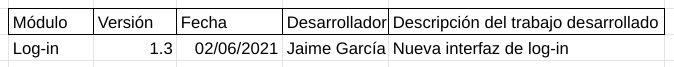
\includegraphics[height=1.3cm]{../images/tabla_versionado_code.png}
   \caption{Tabla de versionado del código.}
   \label{tablaVersionado}
\end{figure}

\begin{figure}[H]
   \centering
       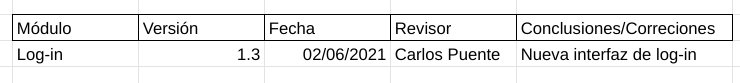
\includegraphics[height=1.5cm]{../images/tabla_conclusiones_revision_pares.png}
   \caption{Tabla de conclusiones de revisión por pares de código.}
   \label{tablaConclusionesPares}
\end{figure}

\pagebreak
\textbf{PL.CA.3: Revisión de los requisitos}

Para comprobar el correcto cumplimiento de los requisitos del sistema se utilizará una tabla de cumplimiento de requisitos (figura \ref{tablaRequisitos}). En este tipo de revisión tanto el desarrollador como el revisor rellenarán dicha tabla y discutirán los resultados. Dichos resultados serán recogidos en una tabla de resumen (figura \ref{tablaConclusionesRequisitos}) que servirá como para futuras revisiones. Los módulos de software a desarrollar anteriormente van asociados a ciertos requisitos del sistema. Antes de comenzar el desarrollo de un módulo se concretarán los requisitos finales a los que hace referencia y se generará la plantilla de la tabla de adecuación de requisitos. Como en el modelo de revisión anterior, cuando el desarrollador del módulo termine una versión importante o realice un avance crítico solicitará una revisión al gestor del proyecto este le asignará un revisor adecuado para la tarea.

\begin{figure}[H]
   \centering
       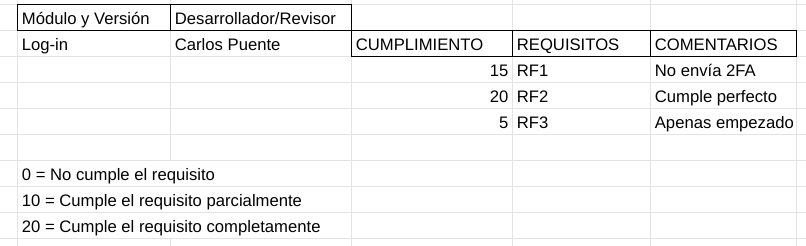
\includegraphics[height=4cm]{../images/tabla_cumplimiento_requisitos.png}
   \caption{Tabla de cumplimiento de requisitos.}
   \label{tablaRequisitos}
\end{figure}

\begin{figure}[H]
   \centering
       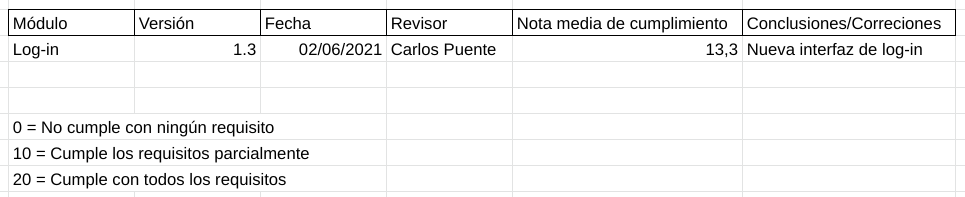
\includegraphics[height=3cm]{../images/tabla_conclusiones_revision_requisitos.png}
   \caption{Tabla de conclusiones de revisión de cumplimiento de requisitos.}
   \label{tablaConclusionesRequisitos}
\end{figure}

Todas estas tablas generadas por el proceso de aseguramiento de la calidad quedarán almacenadas en un directorio remoto accesible por todos los miembros del equipo de desarrollo, agrupadas por el módulo al que hacen referencia de manera que sirvan como histórico de las revisiones realizadas y como mecanismo de monitorización del progreso de las tareas.

\textbf{PL.CA.4: Test sobre el producto}

Para asegurar el funcionamiento correcto del código desarrollado se realizarán pruebas de desarrollo sobre los módulos, las cuales consistirán en pruebas unitarias y pruebas de integración con el resto de componentes del sistema. Además, una vez el sistema sea funcional, se realizarán pruebas globales sobre el sistema, las cuales consistirán en pruebas funcionales, de comunicación, de rendimiento y de sobrecarga. Por último, utilizando las herramientas de despliegue continuo mencionadas anteriormente, se implementarán tests básicos
sobre el sistema previos al despliegue.

\pagebreak

\subsubsection{Calendario del proyecto y división del trabajo} \label{GANTT}

La división del trabajo se consiste en la partición del trabajo en los siguientes módulos:

Módulo de gestión de \textit{sign up} de usuarios, módulo de gestión de \textit{log in} de usuarios, módulo de gestión del \textit{Two-Factor-Authentication}, módulo de generación de contraseñas, módulo de ranking de robustez de contraseñas, módulo de almacenamiento de contraseñas e información por usuario, módulo de búsqueda y ordenación de contraseñas y módulo de gestión y actualización de contraseñas e información. La documentación será del proyecto será actualizada por cada grupo de trabajo usando las \textit{Wikis} de GitHub después de cada sesión de trabajo, de tal manera que los avances realizados en el desarrollo queden registrados haciendo posible el seguimiento del desarrollo al resto del equipo. El diseño gráfico será realizado por todos los miembros del equipo mediante la creación de un \textit{mockup} de la misma en una reunión conjunta. Las instalaciones y los despliegues serán automáticos y continuos mediante \textit{scripts} de GitHub Actions. Las pruebas (Pruebas de desarrollo sobre los módulos y pruebas globales sobre el sistema) se realizarán conforme los desarrolladores vayan terminando sus designaciones y serán los mismos desarrolladores los cuales pasarán las pruebas, en el punto \ref{sec:calidad} se explica en detalle este aspecto.

En la operativa diaria se mantendrá un registro del progreso utilizando la herramienta Trello. Se llevará control sobre las tareas pendientes, en curso y completadas.

Se presenta en la figura \ref{gantt-2} un diagrama de Gantt con el desarrollo previsto del proyecto antes del comienzo de este.

\pagebreak

\begin{landscape}
   \begin{figure}[H]
       \centering
       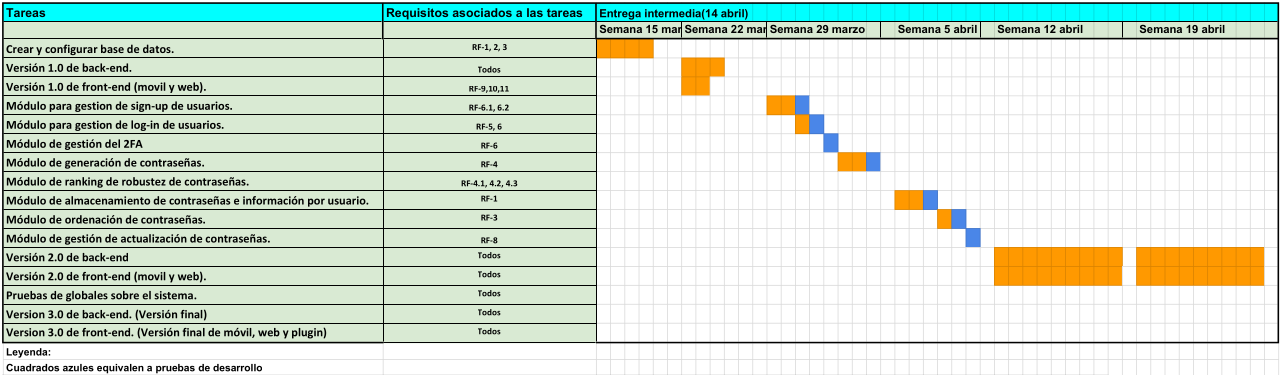
\includegraphics[width=1.4\textheight]{../images/diag-gantt-1.png}
       \label{gantt-1}
   \end{figure}

   \begin{figure}[H]
       \centering
       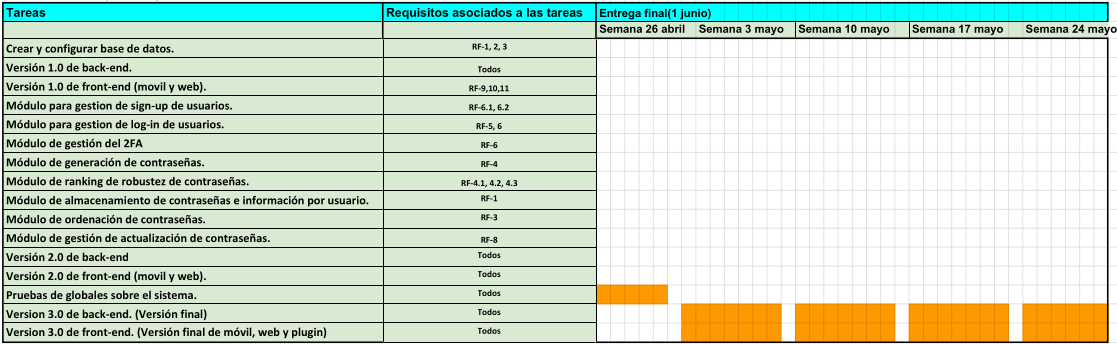
\includegraphics[width=1.4\textheight]{../images/diag-gantt-2.png}
       \caption{Diagrama de Gantt de planificación}
       \label{gantt-2}
   \end{figure}
\end{landscape}

\pagebreak

\section{Análisis y diseño del sistema}

\subsection{Análisis de requisitos}

\begin{table}[H]
   \centering
   \begin{tabular}{| c | p{30em} |}
   \hline
       Código &  Descripción  \\ \hline
       RF-1 & El sistema permite almacenar contraseñas. \\ \hline
       RF-1.1 & El sistema permite almacenar pares que constan de nombre de usuario y contraseña.  \\ \hline
       RF-1.2 & Las entradas de contraseñas tienen un nombre asociado. \\ \hline
       RF-1.3 & El sistema permite asociar a las contraseñas una URL del sitio web al que corresponden. \\ \hline
       RF-1.4 & El sistema registra la fecha de creación o actualización de la contraseña. \\ \hline
       RF-1.5 & El sistema permite almacenar una descripción de texto asociada a la contraseña. \\ \hline
       RF-1.6 & El sistema permite almacenar un único fichero con cualquier extensión asociado a la entrada contraseña. \\ \hline
       RF-1.7 & El sistema permite la creación de contraseñas y la modificación de todos los campos anteriores (nombre, nombre de usuario, contraseña, URL, descripción y fichero). \\ \hline
       RF-2 & El sistema muestra las categorías gestionadas por el usuario. La categoría se define como un directorio donde el usuario almacena contraseñas. Cada contraseña pertenece a una única categoría.\\ \hline
       RF-2.1 & El usuario puede crear, renombrar y eliminar categorías \\ \hline
       RF-3 & El sistema permite visualizar las contraseñas almacenadas\\ \hline
       RF-3.1 & El sistema muestra las contraseñas asociadas a la categoría seleccionada por el usuario. \\ \hline
       RF-3.2 & El sistema muestra los datos y fichero asociados a la contraseña seleccionada. \\ \hline
       RF-3.3 & El sistema permite ordenar las contraseñas de una categoría por fecha de actualización o nombre. \\ \hline
       RF-4 & El sistema permite generación de contraseñas pseudoaleatorias. \\ \hline
       RF-4.1 & El sistema permite seleccionar la longitud de la contraseña a generar.\\ \hline
       RF-4.2 & El sistema permite seleccionar el conjunto de caracteres que compone la contraseña a generar.\\ \hline
       RF-4.3 & El sistema muestra el grado de robustez (entropía) de la contraseña al ser generada. La entropía($E$) se calcula: $E=n\log_2m$. Donde $n$ es la longitud y $m$ el número de caracteres de la población usada.\\ \hline
       RF-5 & El usuario inicia sesión al sistema mediante su correo electrónico y la contraseña maestra. Únicamente podrá acceder con esta contraseña, que no se puede recuperar.\\ \hline
       RF-6 & El sistema requiere autenticación mediante 2FA para iniciar sesión. \\ \hline
       RF-6.1 & El sistema permite el registro de un usuario con: correo electrónico, contraseña maestra y un apodo.\\ \hline
       RF-6.2 & El registro de sesión se deberá confirmar, para verificar la identidad, mediante un correo electrónico a la dirección especificada por el usuario registrado. \\ \hline
       RF-7 & La interfaz de usuario permite copiar al portapapeles del dispositivo la contraseña de una entrada. \\ \hline
       RF-8 & Se accede al sistema mediante una aplicación para dispositivos móviles Android con versión 6.1 (\textit{Marshmallow}). \\ \hline
       RF-9 & Se accede al sistema mediante una aplicación para navegadores web Google Chrome (versión 89) y Firefox (versión 87). \\ \hline
       RF-10 & El sistema ofrece un \textit{plug-in} para el navegador Google Chrome (versión 89). \\ \hline
   \end{tabular}
\end{table}

\subsection{Diseño del sistema}

\subsubsection*{Diagramas de módulos}

\begin{figure}[H]
   \centering
       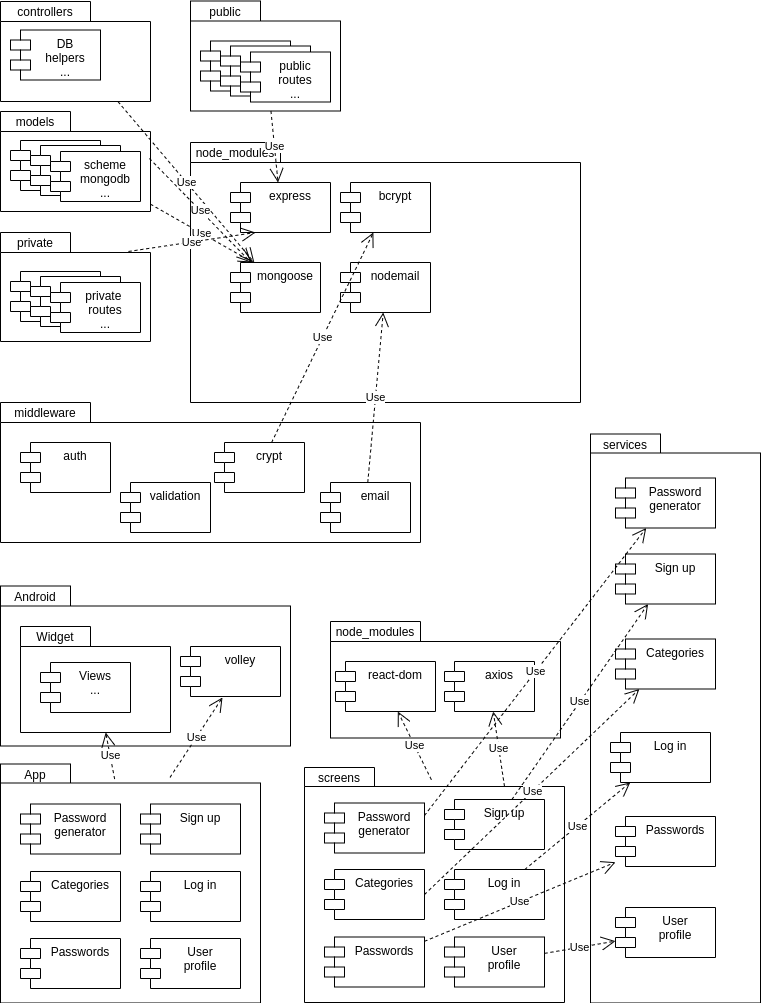
\includegraphics[width=0.99\textwidth]{../images/modulos_v1.png}
   \caption{Diagramas de componentes y conectores.}
   \label{modulos}
\end{figure}
\pagebreak

En el diagrama de módulos en la figura \ref{modulos} se describe las estructuras que el sistema implementa y sus relaciones. Los diferentes paquetes agrupan distintos módulos basándose en su función.

\begin{itemize}
   \setlength{\itemsep}{0em}
   \item 'public': las rutas del modelo accesibles públicamente a través de la API.
   \item 'private': las rutas del modelo que requieren permisos.
   \item 'models': MongoDB \textit{schemes} que modelan la estructura de la información en la base de datos.
   \item 'controllers': colección de módulos que interactúan con la base de datos.
   \item 'middleware': módulos que otorgan funcionalidad variada al sistema.
   \item 'node modules': módulos importados con NPM que ofrecen funcionalidad específica.
   \item 'express': \textit{framework} de desarrollo de servidores web para Node.
   \item 'mongoose': permite la interacción con bases de datos MongoDB.
   \item 'bcrypt': ofrece funcionalidad de cifrado.
   \item 'nodemail': ofrece funcionalidad de envío de correos electrónicos.
   \item 'react-dom': interacción con la vista del navegador web.
   \item 'axios': permite realizar peticiones HTTP al \textit{backend} de la aplicación.
   \item 'screens': vistas del servidor web.
   \item 'services': diferente funcionalidad para la vista de la aplicación.
   \item 'Android': SDK de Android.
   \item 'App': diferentes vistas de la aplicación móvil.
\end{itemize}

Los diferentes módulos externos importados del repositorio de Node o del SDK de Android, ofrecen distinta funcionalidad relativa a las conexiones entre componentes (\textit{e.g. frontend-backend}, \textit{backend}-MongoDB), componentes de vista básicos y seguridad.


\subsubsection*{Diagramas de componentes y conectores}

\begin{figure}[H]
   \centering
       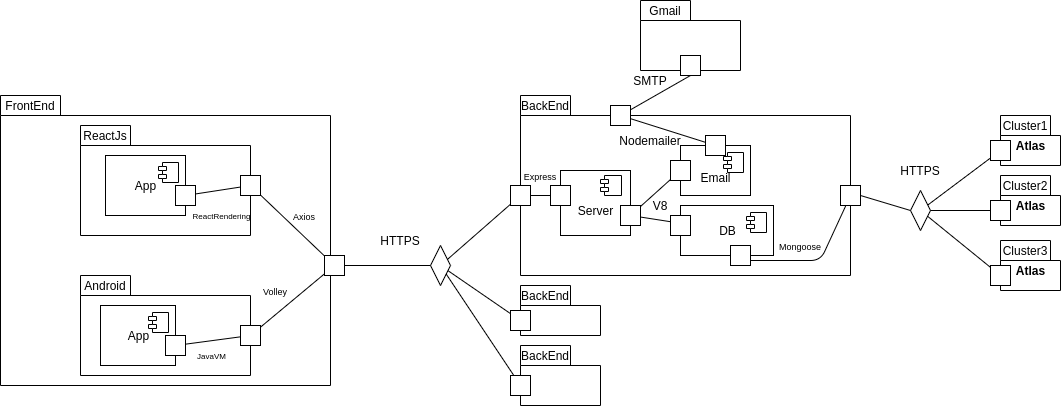
\includegraphics[width=0.90\textwidth]{../images/cyc.png}
   \caption{Diagramas de componentes y conectores.}
   \label{cyc}
\end{figure}

En el diagrama de componentes y conectores en la figura \ref{cyc} se muestra una visión general del sistema, existen tres componentes principales en la aplicación que se relaciona cada uno con una capa del modelo, estos componentes muestran los elementos de presencia en tiempo de ejecución del sistema.

El \textit{frontend} es el componente de la aplicación con el cual el usuario interactúa con el sistema, la aplicación al ser orientada a varias plataformas usa distintos subcomponentes para darle forma a la aplicación, en concreto React.JS, se comunica con el resto de la aplicación mediante el conector React Rendering, De la misma forma lo hace la parte de Android mediante Java Virtual Machine, ambos interaccionan con el resto del sistema usando los puertos que proporcionan las librerías de Axios o Volley.

El conector que relaciona este componente con el componente del \textit{backend} es el protocolo HTTPS a una réplica del servidor.

La interacción entre los componentes del \textit{backend} es más compleja.El puerto que atiende peticiones utiliza Express, y se comunica con los otros componentes usando el motor V8 como conector, que compila en tiempo de ejecución todos los módulos de JavaScript de la parte del servidor. El sistema a su vez tiene un servidor mail que se comunica mediante el protocolo SMTP y que usa la librería Nodemailer para conectar con Gmail. Por último mantendrá una conexión, también usando el protocolo HTTPS, con la base de datos que se encontrará replicada en varios clústeres y alojada en \textit{MongoDB Atlas}, se usa Mongoose para gestionar la conexión con la base de datos.
% Explicar Interfaces de componentes

% Protocolos de comunicación entre componentes

\subsubsection*{Diagrama de distribución}

\begin{figure}[H]
   \centering
       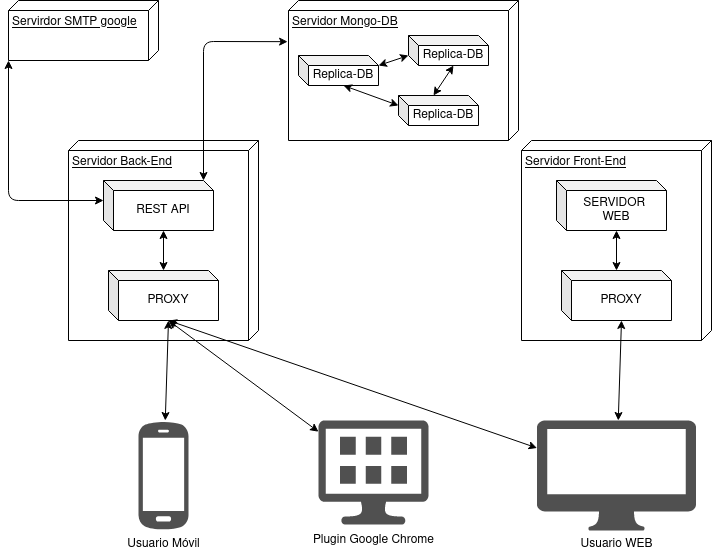
\includegraphics[width=0.99\textwidth]{../images/despliegue2.png}
   \caption{Diagrama de distribución}
   \label{despliegue}
\end{figure}

En el diagrama de despliegue de la figura \ref{despliegue}, se muestra una vista general del sistema en funcionamiento y cómo está distribuido en la nube, en esta vista se asigna cada componente del sistema a un hardware específico.

Tanto el servidor web como el servidor API, se sitúan alojados en los servicios de Amazon AWS y la base de datos se encuentra replicada utilizando MongoDB Atlas.

Se diferencia dos tipos de cliente, el que accede desde un dispositivo móvil y el que accede mediante un protocolo web. El cliente móvil ya tiene compilado el sistema en un dispositivo Android por lo que la capa de acceso a la aplicación este solo tendrá que realizar peticiones directamente a la API REST, a diferencia que el cliente que se conecta mediante un protocolo web, que tendrá en primer lugar que obtener el \textit{template} desde un servidor web para poder realizar peticiones a la API REST.

El servidor cuando requiera realizar operaciones sobre datos persistentes, opera conectándose a un clúster con una réplica de la base de datos MongoDB.

\pagebreak

\subsubsection*{Patrones de diseño y estilos arquitecturales}

A diferencia de la mayoría de \textit{frameworks} que usan el patrón arquitectural modelo vista controlador para separar la lógica de la aplicación de la lógica de vistas, React.JS al ser un \textit{framework} moderno que ofrece \textit{server-side-rendering} por lo que no se puede considerar una arquitectura MVC.
La arquitectura usada (figura \ref{patron}) consiste en tres capas con interfaz web, capa de presentación, capa de negocio y capa datos.

\begin{figure}[H]
   \centering
       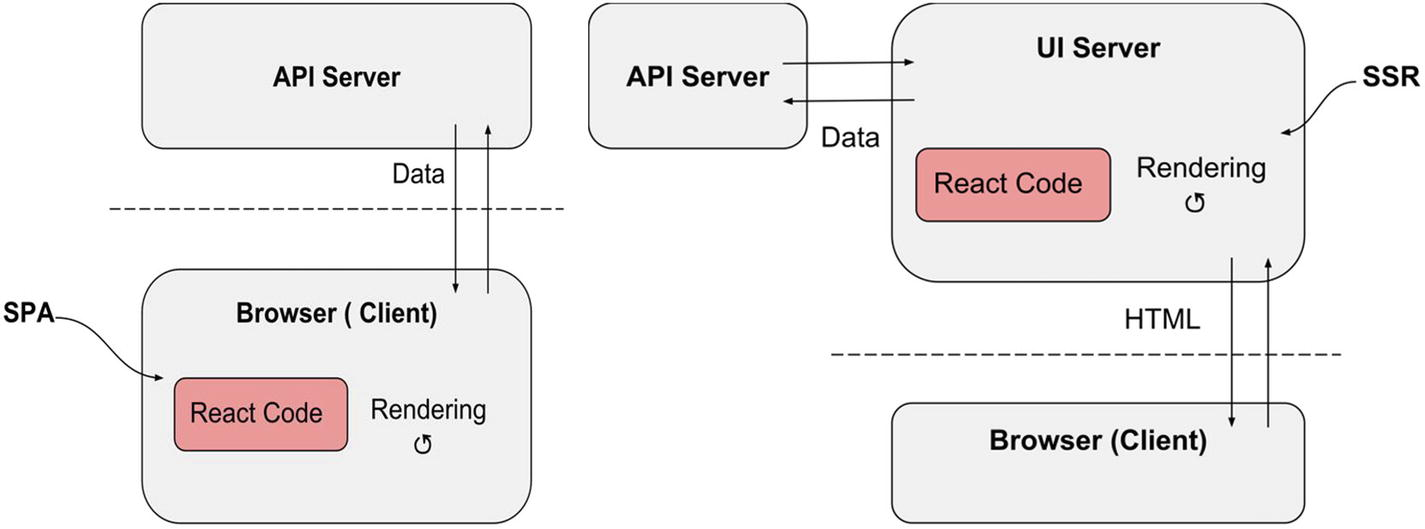
\includegraphics[width=0.99\textwidth]{../images/patron.jpg}
   \caption{Modelo tres capas.}
   \label{patron}
\end{figure}

Como se viene diciendo la capa de presentación o capa de usuario es la que muestra el sistema, le comunica y captura información a la capa de negocio, en esta capa se presentan dos tecnologías Android y React.JS.
La capa de negocio es donde se ejecutan las peticiones del usuario y se envían las respuestas de la ejecución, esta capa se comunica con la capa de presentación para atender a las peticiones y con la capa de datos para almacenar o recuperar datos. Para esta capa se utilizará el entorno de ejecución Node.
La capa de datos es la encargada de almacenar los datos mediante en gestor de base de datos, en el caso de la aplicación se utiliza la base de datos no relacional MongoDB.


\subsubsection*{Tecnologías elegidas}

Se hará uso de lenguajes de programación como JavaScript para la interfaz web (React) y para el modelo (Node). Es la tecnología requerida por el \textit{stack} de lenguajes para aplicaciones web MERN. Es sencillo, debido a su conocimiento previo, y unifica la tecnología para el desarrollo \textit{backend} y \textit{frontend}.

La aplicación móvil se desarrollará en Java (Android), que permite desarrollo nativo para teléfonos, es ampliamente utilizado y se conoce de proyectos anteriores. Se propuso el uso del entorno React Native, pero se descartó debido a su desconocimiento por parte del grupo.

El componente de la vista de la aplicación se conecta a la API del modelo para realizar peticiones relativas a la acción del usuario. Esta segunda se conecta con la base de datos MongoDB en los servidores Atlas de Mongo. Se prefiere el uso de Atlas frente al despliegue de la base de datos en una máquina virtual debido a su facilidad de administración y la disponibilidad ofrecida.

\pagebreak

La base de datos MongoDb es NoSQL y, frente a una base de datos SQL como Oracle, permite más flexibilidad para recoger y persistir información. Además, MongoDB junto a Mongoose, ofrecen facilidad de interacción con JavaScript mediante ficheros JSON.

Para la creación de la API web ofrecida por el servidor del modelo, se ha optado por seguir la estructura API REST, que es ampliamente utilizada y fácil de implementar con las tecnologías utilizadas.

La tecnología Node hace uso de un bucle de eventos el cual permiten la realización de operaciones asíncronas para realizar peticiones en el \textit{background} y recibir respuestas sin necesidad de interrumpir la operativa esperando a esta.

Se ha optado por utilizar el módulo Bcrypt para cifrar los datos de la aplicación y utilizar el protocolo HTTPS para asegurar las comunicaciones.

\pagebreak

\section{Memoria del proyecto}

\subsection{Inicio del proyecto}

En la identificación y asignación de recursos a utilizar, se ha decidido basándose en los conocimientos tecnológicos de cada integrante del grupo y el grado de familiarización con las tecnologías.

Respecto a los servidores en \textit{cloud} a utilizar para el despliegue del sistema, el criterio de elección se ha basado en el estudio del impacto a nivel global de la empresa, es decir, grado de utilización en el mundo empresarial y la cantidad de servicios ofrecidos gratuitamente. Finalmente, se decidió crear una cuenta en AWS, siendo así Amazon el proveedor de \textit{cloud} para el proyecto.

En relación con la base de datos, se ha decidido usar una base no relacional debido al grado de flexibilidad del modelo de datos que ofrece frente al modelo típico relacional. Como SGBD se ha escogido MongoDB. Se ha creado una cuenta en MongoDB Atlas el cual permite crear una base de datos remota accesible por el sistema.

En cuanto a la formación inicial de los integrantes, se han tenido en cuenta en el reparto de responsabilidades los conocimientos de los desarrolladores, sin embargo, todos los desarrolladores han dedicado tiempo de manera individual en autoformación y documentación sobre las tecnologías a usar en el desarrollo del sistema. Además, todos los integrantes del grupo se han comprometido a formar a sus compañeros en las áreas que conozcan a medida que surjan dudas durante el desarrollo del sistema.

\subsection{Ejecución y control del proyecto}

Las comunicaciones entre los miembros del grupo de trabajo se han realizado principalmente a través de la herramienta de comunicación WhatsApp, mediante la cual se concretan los horarios de trabajo y se informa acerca de actualizaciones puntuales en las tareas asignadas a cada miembro para que todo el equipo quede informado de cómo avanzan los distintos componentes del trabajo. Además, las reuniones semanales de puesta en común del trabajo se han realizado utilizando la herramienta de videoconferencia Google Meet. Esta última será el principal medio de comunicación del grupo. Destacar que pese a la división de trabajo previo, se intenta trabajar de manera conjunta por videoconferencia, de manera que se puedan poner en común y resolver problemas en la medida en que surjan.

El registro de las decisiones tomadas en las reuniones, se ha realizado mediante actas de cada una de ellas. El almacenamiento de estas actas se realiza en un directorio remoto en GitHub.

Partiendo de la división inicial del grupo en equipos de trabajo detallada en el punto \ref{sec:organizacion}, los responsables de cada equipo de trabajo se han encargado de monitorizar el avance de sus respectivos módulos, determinar las tareas a realizar, asignar dichas tareas a los desarrolladores y marcar límites temporales y prioridades para cada tarea. En cuanto al trabajo de documentación de los avances sobre el código, todos los desarrolladores han sido los responsables de registrar los mismos en las \textit{wikis} de GitHub habilitadas para ello en cada repositorio de código. Así mismo, los desarrolladores han rellenado una tabla de control de esfuerzos para registrar su trabajo y cumplir con el resto de planes especificados más adelante.

\pagebreak

Respecto a la monitorización y control del progreso del proyecto, todas las semanas se ha realizado una reunión conjunta de control en una hora y día fija a la cual asisten todos los miembros del grupo para exponer los avances realizados durante la semana y poder determinarse el estado del proyecto y las siguientes tareas a desarrollar.

La entrega de resultados se realiza de manera continua de forma que el cliente pueda ir viendo el progreso del proyecto. Los resultados finales, que contendrán los códigos fuente, \textit{scripts} de compilación y despliegue, etc. también serán entregados al cliente.

Para implementar las vistas del sistema se ha utilizado por una parte Java (Android SDK) para construir el cliente móvil para dispositivos Android y por otra JavaScript (React.JS) para desarrollar el \textit{frontend} web. En cuanto al \textit{backend}, se ha desarrollado utilizando Node.JS y el \textit{framework} Express. La base de datos utilizará el SGBD MongoDB. El despliegue del sistema se realizará en un entorno de contenedores Docker desplegado sobre máquinas virtuales en \textit{cloud}. Se seguirá una filosofía de entrega y despliegue continuo utilizando \textit{scripts} y GitHub Actions.

\subsubsection*{Ejecución de los planes:}

\textbf{PL.I.1:}
Se ha escogido como proveedor \textit{cloud} Amazon AWS. Esta decisión ha permitido desde el principo disponer de una plataforma \textit{cloud} gratuita para el despliegue, no se han recibido cobros inesperados por parte del proveedor y se ha mantenido en todo momento la disponibilidad de las máquinas virtuales. En ningún momento a lo largo del proyecto se ha planteado cambiar esta decisión. Se concreta por tanto que ha el plan cumplido con su objetivo.

\textbf{PL.I.2:}
Para la implementación del modelo de datos, se ha escogido el SGBD MongoDB. Este SGBD administra bases de datos no relacionales, que se caracterizan por su flexibilidad. La decisión se considera correcta, el equipo de desarrollo de Back-End considera que ha sido fácil trabajar con este gestor gracias a su extensa documentación y la disponibilidad de librerías para su manipulación en Node.js. El gestor ha dado soporte para almacenar correctamente todos los datos del sistema y ha asegurado una correcta disponibilidad y consistencia de los mismos. Se concreta por tanto que el plan ha cumplido con su objetivo.

\textbf{PL.I.3:}
El plan de formación inicial de los desarrolladores ha sido uno de los más dificiles a llevar a cabo. Aunque todos los desarrolladores han cumplido con el plan y dedicado su tiempo personal a familizarse con las nuevas tecnologías, la mayor parte de la familiarización y el aprendizaje se ha desarrollado a medida que se implementaban los distintos módulos. Por tanto, como posible mejora para futuros proyectos, se propone asignar a los desarrolladores pequeñas tareas de desarrollo utilzando las tecnologías a aprender, para asegurar un grado de familiarización con las tecnologías previo al desarrollo del proyecto.

\textbf{PL.EC.1:}
El plan de comunicación se ha cumplido tal y como se había especificado y ha cumplido su objetivo permitiendo en todo momento una comunicación fluida y una correcta sincronización entre los integrantes del proyecto.

\textbf{PL.EC.2:}
El plan de realización de reuniones de todos los integrantes del proyecto ha resultado muy beneficioso, todos los integrantes han acudido y participado en las reuniones permitiendo al director del proyecto conocer de primera mano el estado de desarrollo de los distintos módulos permitiendo por tanto tomar las decisiones de control pertinentes.
Además, se ha llevado a cabo correctamente el registro de las decisiones tomadas. Javier Vela, el responsable de este proceso, ha cumplido con su cometido y registrado en todas las reuniones las decisiones tomadas. Tener este histórico de decisiones, también ha permitido a los desarrolladores acceder a estas en momentos puntuales en los que se necesitaba cierta información. Por útltimo, la monitorización de avance semanal, ha permitido mantener correctamente un control del avance del desarrollo, asignar tareas a los desarrolladores y marcar limites temporales y prioridades de las tareas, se concluye por tanto que ha sido efectivo y útil.

\textbf{PL.EC.3}
El plan de documentación del código no se ha seguido tal y como se había como se había planteado. El equipo de Back-End si que ha utilizado las wikis de github para documentar el modo de uso de la REST API implementada y para documentar el proceso de configuración de las máquinas virtuales para el despliegue. Sin embargo, los equipos de Front-End no han utilizado las wikis para llevar a cabo la documentación del código sino que han realizado este trabajo mediante comentarios en el propio código. Como mejora se propone cambiar el plan y definir un convenio de documentación del código utilizando comentarios de tal manera que el uso de las wikis sea opcional para los casos en los que tenga utilidad (como en el caso del Back-End). Se confirma por tanto que el plan no ha sido útil al 100\%.

\textbf{PL.EC.4}
El control de los esfuerzos realizados por los desarrolladores se ha desarrollado conforme se había establecido en los planes, la tabla de control ha resultado de gran ayuda para comprobar el avance del trabajo. También se ha utilizado para que los desarrolladores fuesen conscientes del tiempo empleado y para poder hacer una valoración final del tiempo empleado en el proyecto.

\textbf{PL.EC.5}
El plan de entrega de resultados continuo se ha seguido tal y como se había planteado siguiento la filosofía de despliegue continuo del sistema, estando disponible en todo momento del desarrollo una versión en producción de los distintos componentes del sistema.

\textbf{PL.EC.6}
EL plan de nombrado de archivos ha probado ser útil para comprender la disposición del código y asegura la navegabilidad del mismo cumpliendo por tanto su objetivo. Ha sido respetado por todos los desarrolladores, resultando ser intuitivo a la hora de ser utilizado mientras se desarrolla. Como problema podría destacarse que en el entorno de Express ha sido menos intuitivo utilizar la convención de nombrado, ya que normalmente los archivos se nombran comenzando por minúscula.

\textbf{PL.EC.7}
El plan de estructurado de directorios cumplido su objetivo habiendo ayudado a los desarrolladores a mantener una correcta estructura de código en los distintos subproyectos y ayudando a su vez la navegabilidad y comprensión del código.

\textbf{PL.EC.8}
Los desarrolladores del proyecto se han valido de las guías de estilo recomendadas por el plan de uso de guía de estilo, acudiendo a ellas a la hora de implementar código.

\textbf{PL.EC.9}
El plan de control de versionado y actualización del código ha resultado ser muy útil para mantener el código accesible para todos los desarrolladores. Se destaca que la herramienta GitHub ha permitido a los desarrolladores ver el código del resto de los integrantes del código, asegurar que el código no se pierda, acceder a versiones de código anteriores para comprobar configuraciones anteriores y mantener un régimen de despliegue y entrega continuos. La herramienta y el uso de esta ha sido adoptada por todos los integrantes del proyecto sin ningún problema, destacando todos ellos su facilidad y comodidad de uso.

\textbf{PL.EC.10} %REVISAR TODO ESTE Punto...
En el ámbito del plan de aseguramiento de la calidad, el plan de uso de guías de documentación y de diseño gráfico ha resultado más difícil de aplicar que el resto de planes. En cuanto al uso de guía de documentación, los desarrolladores han consultado las tendencias del mercado para basarse en ellos a la hora de completar la documentación. Sin embargo se ha escogido documentar el código sin seguir estrictamente estándares especificos buscando un estilo comprensible por todos los integrantes del proyecto. Respecto a las guías de diseño gráfico, los desarrolladores de los componentes de \textit{frontend} se han asegurado de diseñar las vistas de usuario de forma que sean claras, simples y fáciles de usar por los usuarios futuros.

El plan de revisión de código por pares ha sido llevado a cabo por los desarrolladores tal y como se había estipulado. Ha resultado ser útil para mantener un control del avance y la calidad del código. Sin embargo, se prevé que su utilidad crezca en la segunda iteración del proyecto a medida que vayan creciendo los registros de las revisiones.

EL plan de revisión de requisitos ha sido llevado a cabo por los desarrolladores tal y como se había estipulado.
Se ha comprobado su utilidad a la hora de mantener el control sobre el avance de los requisitos, asegurando que ningún requisito queda sin implementarse. Sin embargo, se prevé que su utilidad crezca en la segunda iteración del proyecto a medida que vayan creciendo los registros de las revisiones pudiendo comprobarse el avance real del proyecto.

El plan de test sobre el producto ha permitido asegurar la corrección de los distintos módulos a la vez que se desarrollaban permitiendo detectar bugs antes de integrarlos con el resto de componentes del sistema. En la segunda iteración se desarrollarán las pruebas generales previstas sobre el producto completo.

\textbf{PL.T.1}
%PENDIENTE%

\textbf{PL.T.2} %PENDIENTE%

\textbf{PL.T.3}
El plan de definición del modelo de datos se ha cumplido tal y como se había definido y a tiempo asegurando desde el principio un modelo de datos adecuado para almacenar la información del sistema.

\textbf{PL.T.4} %PENDIENTE%


\textbf{PL.T.5}
El sistema se encuentra desplegado en su totalidad sobre dos máquina del servicio de \textit{Amazon Web Services}, y se puede acceder a las rutas de la REST API solo a través del puerto 443 (puerto HTTPS) redirigiendo las peticiones del puerto 80 al 443 para mantener la confidencialidad. Estas peticiones son reexpedidas usando el \textit{reverse proxy} Nginx, para asegurarse una conexión segura el \textit{proxy} obtiene el certificado digital mediante la entidad certificadora Let's Encrypt, que proporciona certificados de forma gratuita.
Entre las principales desventajas que conlleva usar el servicio gratuito de \textit{Amazon Web Services} es que no ofrece una IP estática para la máquina, por ello se ha tenido que utilizar el servicio gratuito no-ip que proporciona dominios a Ip's de forma dinámica, lo que provee a las máquinas cliente y servidor, de dos nombres DNS por las que se les puede identificar. La máquina servidor(\textit{backend}) está bajo el nombre del dominio \textit{https://keypax-api.sytes.net} y la máquina cliente(\textit{frontend}) está bajo el nombre \textit{https://keypax.sytes.net}.




\subsection{Cierre del proyecto}

\subsubsection*{Análisis del seguimiento del calendario del proyecto}

En la Figura \ref{gantt-3-n} se compara el desarrollo del proyecto planificado en la sección \ref{GANTT} frente al desarrollo real. Las principales diferencias radican en que, mientras que en la planificación inicial se previó un desarrollo por versiones cada vez más complejas; en realidad, se produjo un avance módulo por módulo y una integración continua permitiendo validar el funcionamiento de cada uno de ellos tras su finalización.

El desarrollo conjunto entre todos los equipos de los módulos correspondientes no ha podido ser posible, ya que ciertas tareas necesitaban más tiempo que otras para algunos equipos. Se ha seguido una implementación independiente entre los equipos para no impedir el avance de algún otro equipo a la espera de la terminación de otro.

En la imagen comparativa se puede observar (en naranja claro) el desarrollo previsto para la primera versión, el cual solo el equipo de \textit{backend} pudo llevar al día. Los otros equipos, tras asentar las tecnologías a utilizar, comenzó el trabajo con un desfase inesperado. Pese a que el avance del proyecto en la parte final de este ha sido más rápido de lo esperado y se ha completado en menos tiempo del planificado, el desajuste con el horario planificado ha creado incertidumbre en el equipo sobre el cumplimiento o no de la temporización.

Las pruebas del sistema fueron planificadas al terminar cada una de las tres versiones del proyecto. En realidad, las pruebas de cada uno de los módulos, de la integración entre estos y la validación en el entorno de producción fueron realizadas con continuidad al terminar distintas fases.

\begin{landscape}
   \begin{figure}[H]
       \centering
       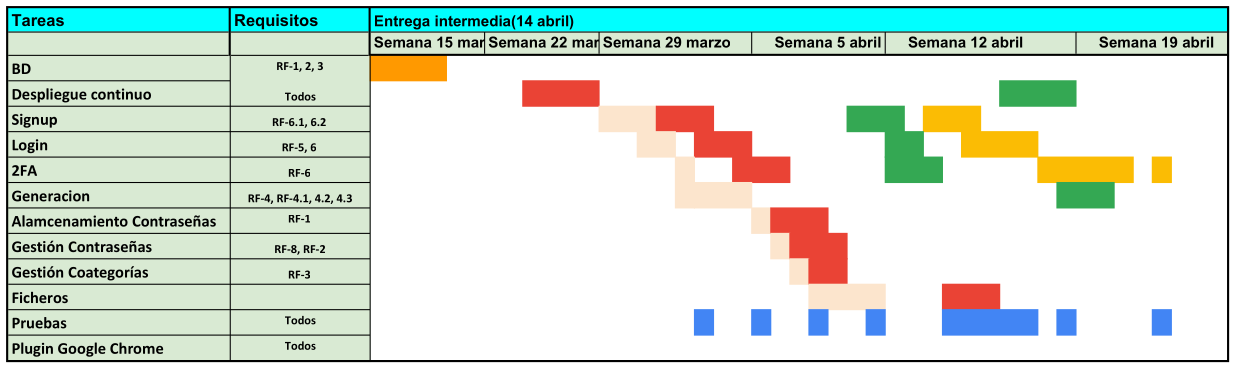
\includegraphics[width=1.2\textheight]{../images/diag-gantt-1-nuevo.png}
       \label{gantt-1-n}
   \end{figure}

   \begin{figure}[H]
       \centering
       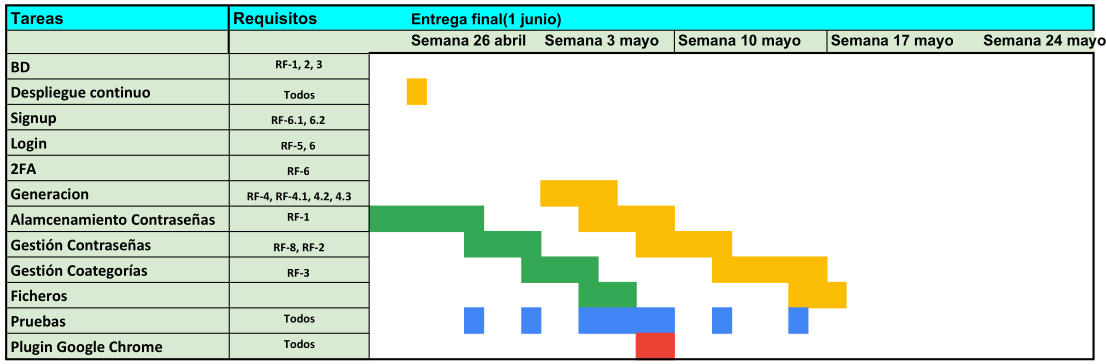
\includegraphics[width=1\textheight]{../images/diag-gantt-2-nuevo.png}
       \label{gantt-2-n}
      \end{figure}

      \begin{figure}[H]
         \centering
         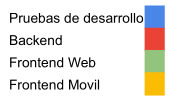
\includegraphics[width=0.2\textheight]{../images/diag-gantt-3-nuevo.png}
         \caption{Diagrama de Gantt de la realización del proyecto}
         \label{gantt-3-n}
  \end{figure}
\end{landscape}
\pagebreak

\subsubsection*{Recopilación de esfuerzos}

Se va a realizar un análisis del esfuerzo en tiempo realizado por los miembros del equipo partiendo del número de horas dedicadas a la realización del proyecto desde las tres perspectivas en las que se ha dividido el trabajo.

Para el conteo del número de horas, cada miembro del equipo contaba con una hoja excel individual donde se anotaba el número de horas dedicadas a una determinada tarea junto a la fecha de realización y una descripción.

\begin{itemize}
  \item Para la total finalización de la API REST de keypax se han utilizado un total de 119 horas.
  \item Para completar la aplicación móvil se han empleado en total 144 horas.
  \item Para puesta en marcha del servicio web de KeyPaX se han empleado 129 horas.
  \item Para el despliegue de la extensión de Google Chrome se han necesitado 15 horas.
\end{itemize}

En total el número de horas dedicadas a gestión del proyecto software lo que incluye memorias, reuniones con el equipo y con el tutor y la fase de preparación del proyecto asciende a 61,5 horas. Lo que en conjunto suman un total de 468,5 horas dedicadas al proyecto.


\subsubsection*{Análisis de rentabilidad del tiempo invertido}

Durante la fase de preparación del proyecto se llevó a cabo una estimación del tiempo que se requería para la completa finalización del proyecto, con la finalidad de realizar una propuesta económica, en la que se estimó el tiempo necesario para la realización de cada módulo que compone el sistema, y se ajustó un presupuesto concorde al tiempo aproximado que se había estimado.

La propuesta acordaba una media de 842 horas invertidas en el proyecto divididas entre 305 horas de backend en las que se engloba tanto desarrollo como documentación, 360 horas acordadas para la finalización del frontend junto a 29,5 más de diseño de la interfaz del sistema, Y 147,5 horas dedicadas a la prueba del sistema y cada módulo que lo compone.

En dicho análisis se sobreestimó por bastante el coste de horas que se deberían dedicar al proyecto, mayoritariamente en el coste en tiempo de desarrollo del servidor del sistema. Al ser el tiempo invertido en proyecto inferior a la máxima estimación propuesta se puede afirmar que la rentabilidad de la aplicación ha sido alta. En concreto el coste del proyecto alcanza el valor de 8.667,25€, por lo que el beneficio del proyecto asciende a la cantidad de 11.270€

\subsubsection*{Conocimientos sobre herramientas y tecnologías adquiridos}

Para la realización del proyecto los diferentes equipos de desarrollo se han tenido que enfrentar a diversas dificultades, la mayor sin duda alguna ha sido la adaptación a las nuevas tecnologías, donde los distintos miembros del equipo se han tenido que documentar a la perfección para llevar a cabo un desarrollo inteligente y efectivo, esta adversidad sin embargo no solo ha conllevado un gasto de horas, sino que también ha aportado una \textit{mochila de conocimientos} que serán de utilidad para afrontar con mayor facilidad próximos proyectos.

El equipo del frontend nunca antes había trabajado con un framework como ReactJs, de hecho sus conocimientos web en HTML y CSS eran básicos. A lo largo del proyecto se han logrado adaptar adquiriendo altos conocimientos en desarrollo de páginas web dinámicas y \textit{Responsive} a través del uso de la librería \textit{Material UI} que facilitaba la estilización de componentes.

El equipo móvil tenía una breve experiencia en el desarrollo de aplicaciones nativas en Android sin embargo nunca se habían enfrentado a un problema de tanta envergadura, adquiriendo significativos conocimientos en estilización con XML, además de aprender a gestionar sesiones seguras desde dispositivos Android.

El equipo backend ya gozaba de experiencia en desarrollo de servidores por lo que el nivel de conocimiento adquirido ha sido menor, sin embargo se ha trabajado con bases de datos no relacionales de las cuales el conocimiento era básico. Además se ha cogido soltura con la implementación de distintos algoritmos de cifrado tanto para proteger las contraseñas de los usuarios como para encriptar ficheros.



\pagebreak

\section*{Conclusiones}
\addcontentsline{toc}{section}{Conclusiones}

Se concluye el proyecto obteniendo un producto robusto y fiable. Es un sistema fácil y cómodo de usar en el día a día para la gestión de contraseñas. Cumple todo lo acordado con el cliente en la propuesta inicial y satisface todos los requisitos. Se ha reforzado la idea de la complejidad involucrada en un proyecto de mayor tamaño y, por ello, la necesidad de planificación. Se ha reforzado el trabajo en grupo entre los compañeros y se ha destacado la necesidad de comunicación entre todos los equipos involucrados en el desarrollo de un mismo producto. El equipo se encuentra satisfecho con el producto final, el desarrollo y el resultado del proyecto.

\subsection*{Posibles mejoras observadas}

Se han detectado posibles mejoras que, en un futuro proyecto, con el mismo equipo u otro diferente, para el desarrollo de un producto similar; permitiesen elaborarlo con más funcionalidad, menos problemas y en un tiempo menor.

\begin{itemize}
   \setlength\itemsep{0em}
   \item Los procesos y planes especificados para este proyecto pueden ser reutilizados sin necesidad de una nueva definición, ya que son generales y se pueden aplicar a cualquier proyecto inicial.
   \item El uso de las tecnologías de este proyecto permite reducir el tiempo de descubrimiento y aprendizaje.
   \item Planificar un despliegue continuo desde el principio, facilitando la integración y pruebas del sistema. Se puede utilizar el mismo sistema de GitHub Actions.
   \item Hacer equipos más equilibrados, ahora que todos tenemos un conocimiento de la tecnología más general, para permitir un avance más controlado.
   \item
\end{itemize}

\pagebreak

\section*{Glosario}
\addcontentsline{toc}{section}{Glosario}

\section*{Bibliografía}
\addcontentsline{toc}{section}{Bibliografía}

\section*{Anexo I. Actas de reuniones realizadas con el tutor}
\addcontentsline{toc}{section}{Anexo I. Actas de reuniones realizadas con el tutor}
\begin{figure}[H]
   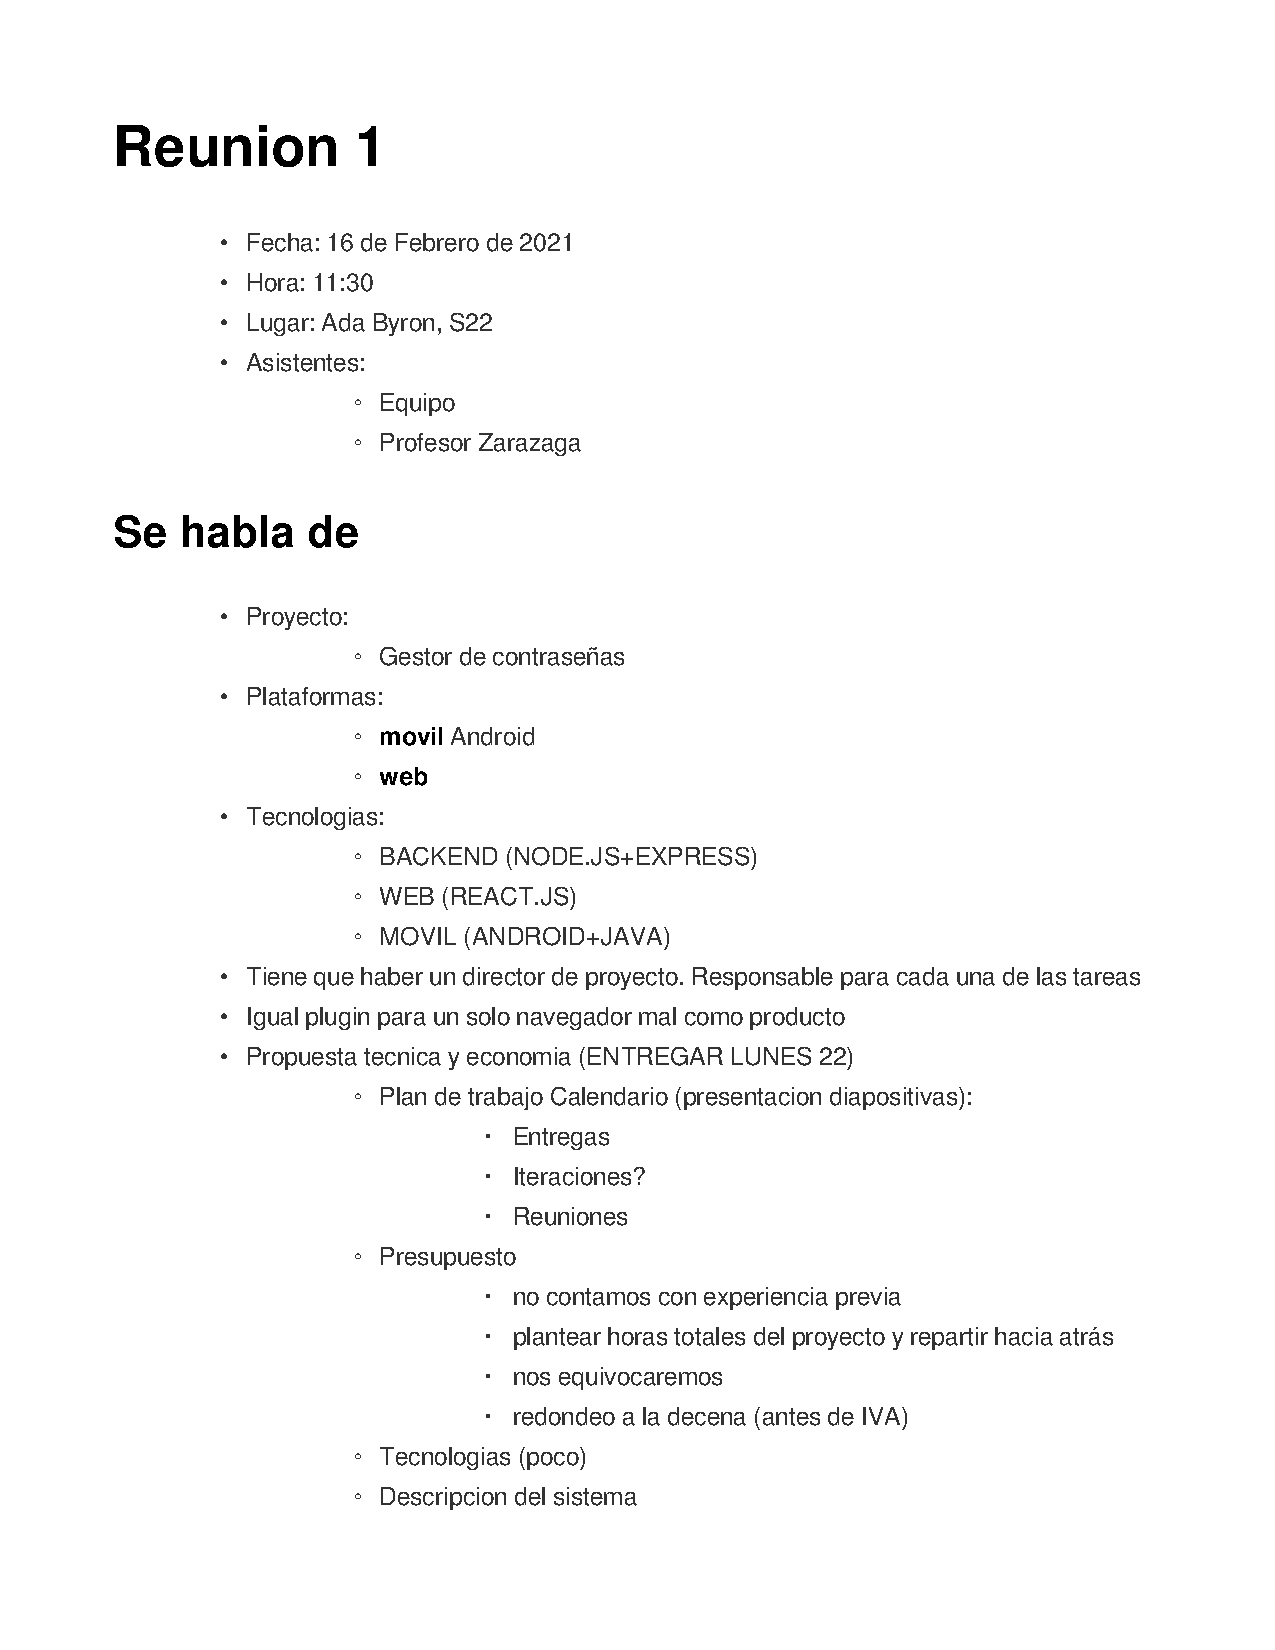
\includegraphics[width=.8\textwidth]{../../actas_reuniones/2021.02.16_1_Actas.pdf}
   \caption{Acta 1 16/02/2021}
\end{figure}
\begin{figure}[H]
   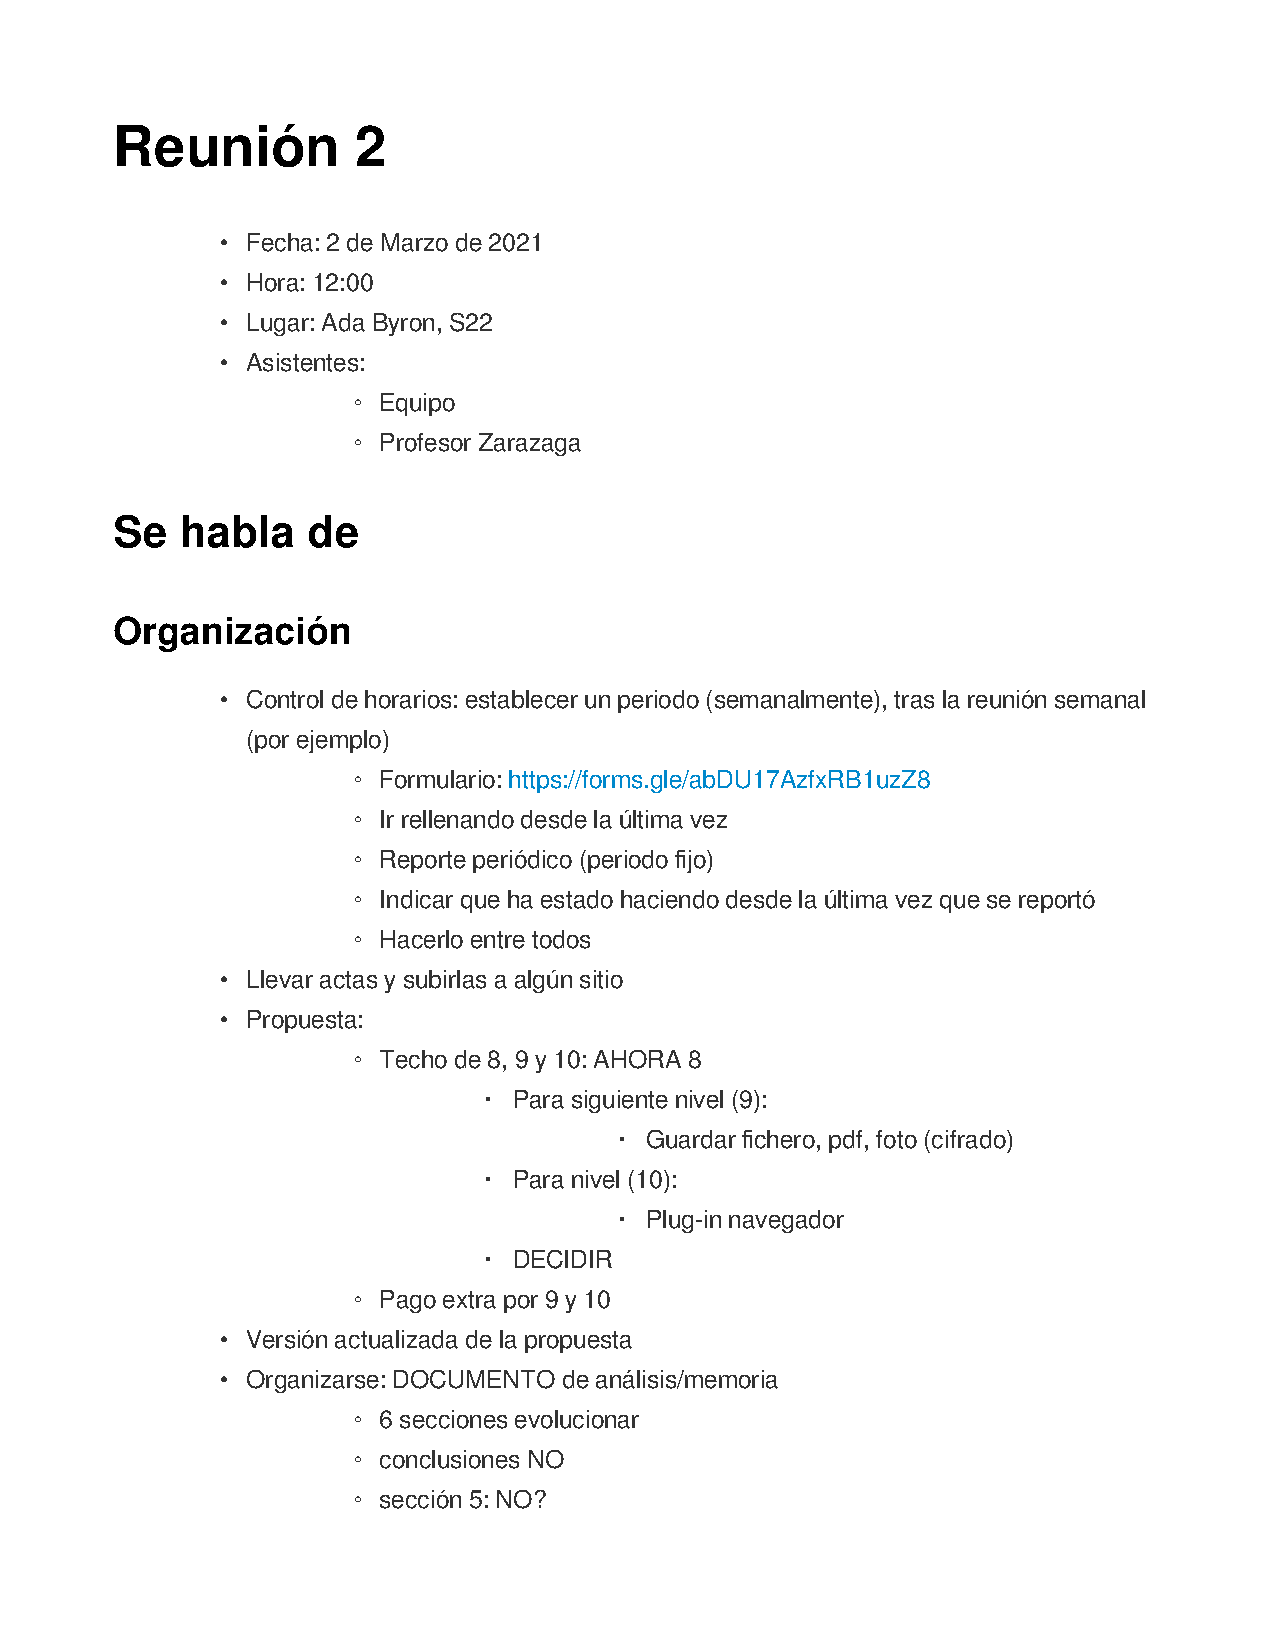
\includegraphics[width=.8\textwidth]{../../actas_reuniones/2021.03.02_2_Actas.pdf}
   \caption{Acta 2 02/03/2021}
\end{figure}
\begin{figure}[H]
   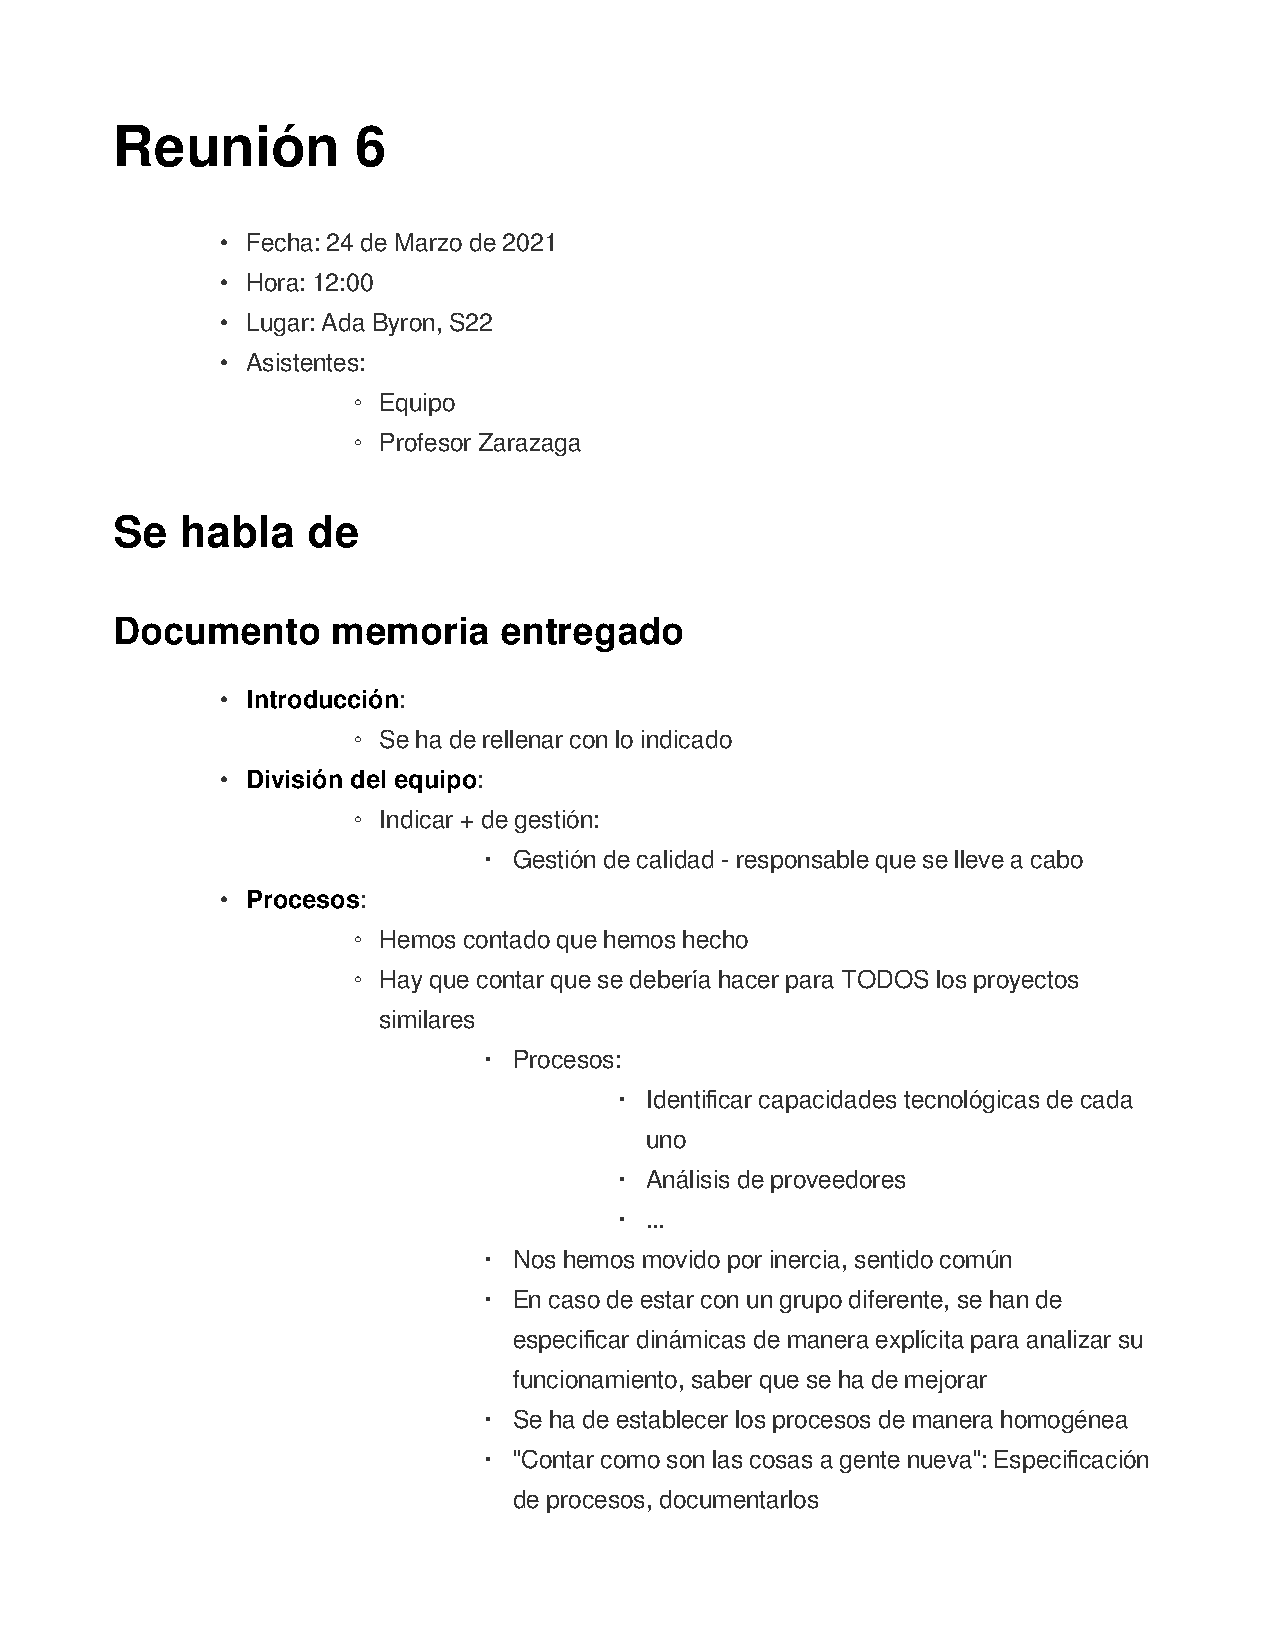
\includegraphics[width=.8\textwidth]{../../actas_reuniones/2021.03.24_3_Actas.pdf}
   \caption{Acta 3 24/03/2021}
\end{figure}
\begin{figure}[H]
   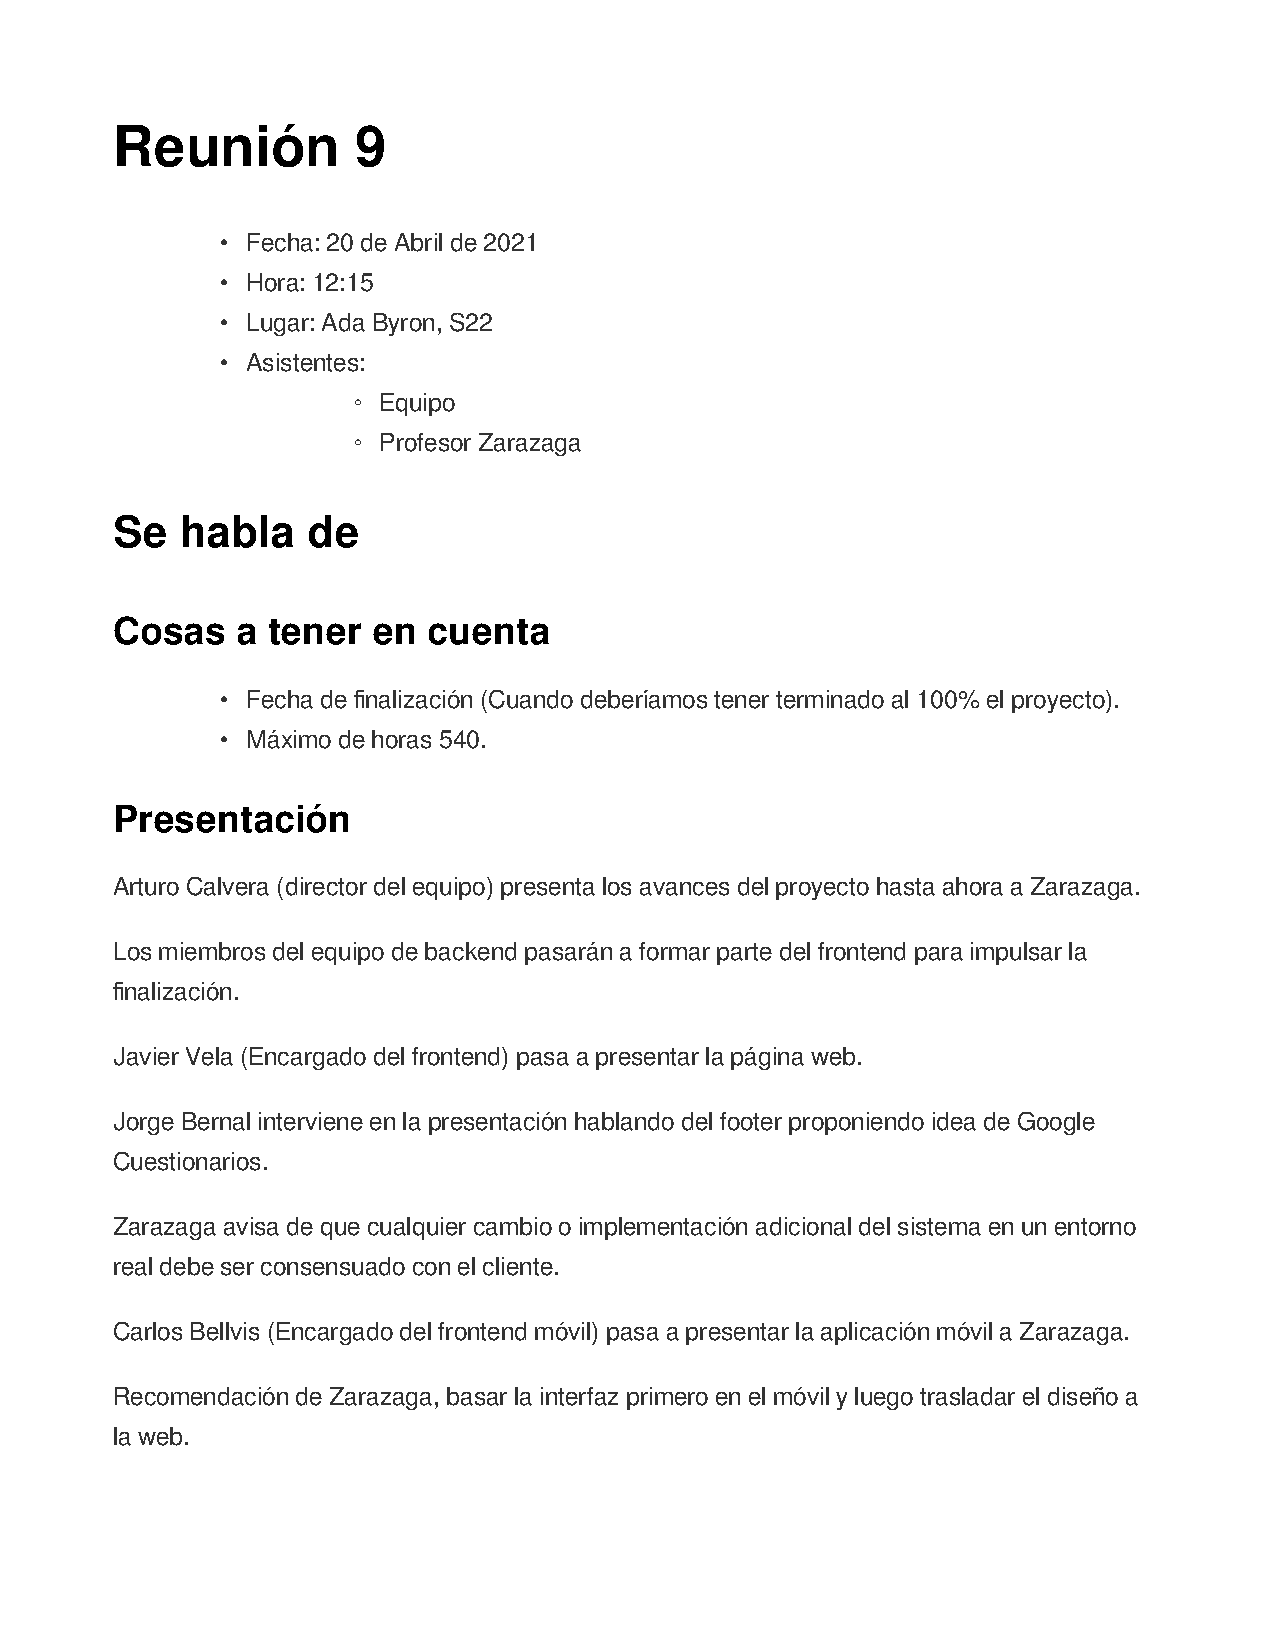
\includegraphics[width=.8\textwidth]{../../actas_reuniones/2021.04.20_4_Actas.pdf}
   \caption{Acta 4 20/04/2021}
\end{figure}
\begin{figure}[H]
   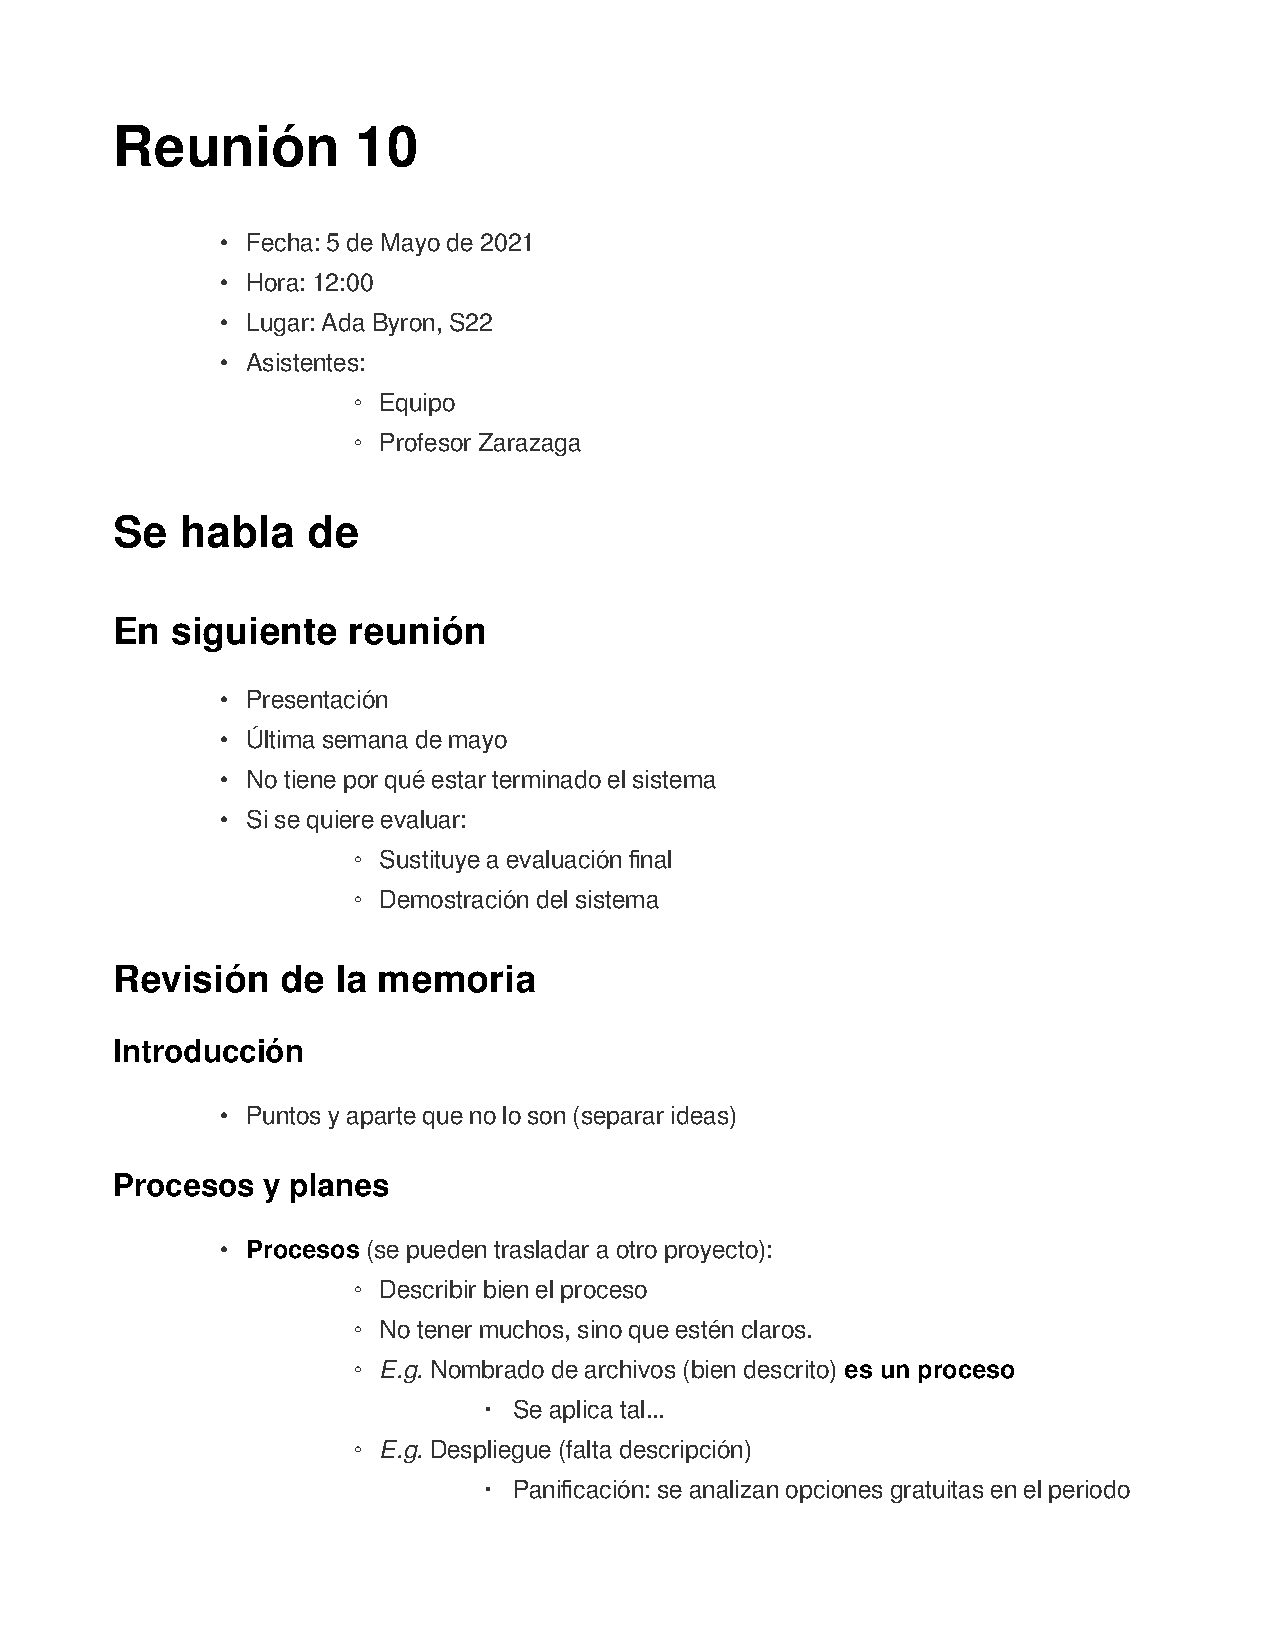
\includegraphics[width=.8\textwidth]{../../actas_reuniones/2021.05.05_5_Actas.pdf}
   \caption{Acta 5 05/05/2021}
\end{figure}
\begin{figure}[H]
   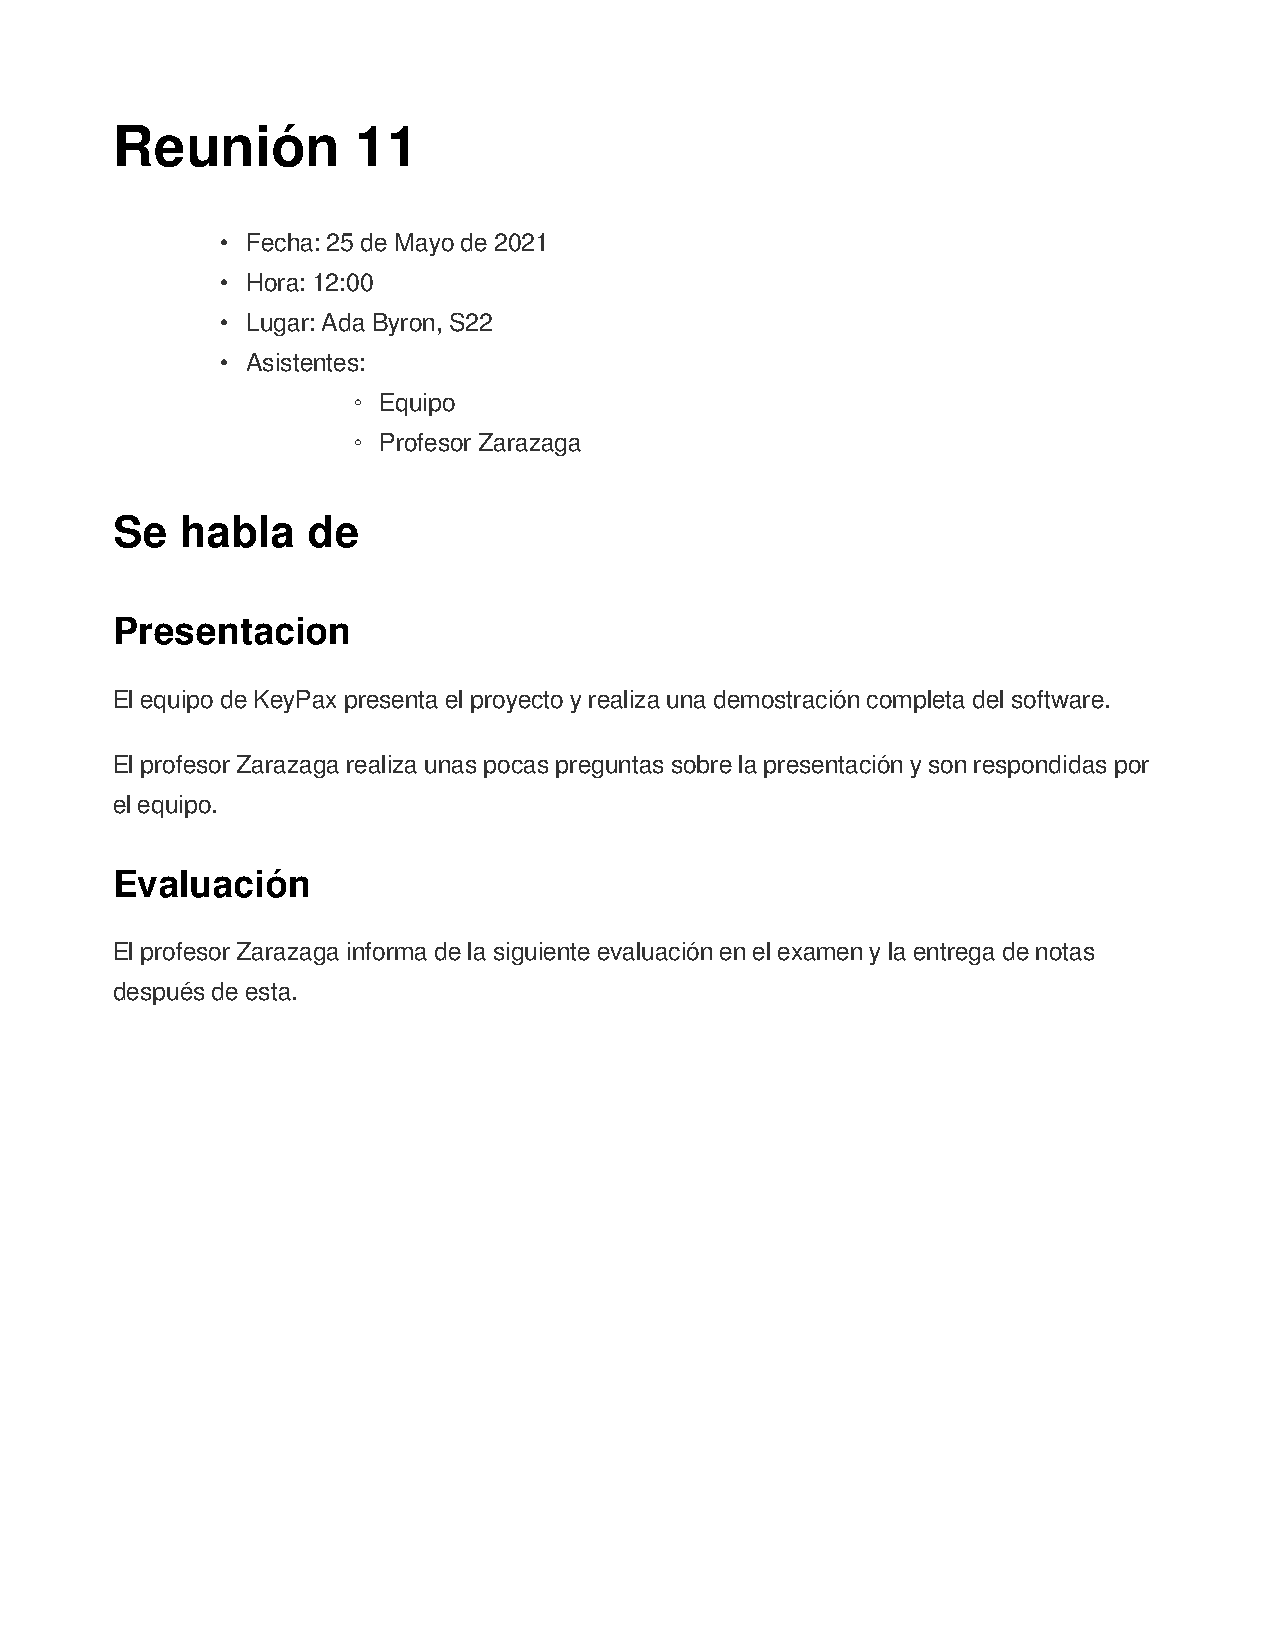
\includegraphics[width=.8\textwidth]{../../actas_reuniones/2021.25.05_6_Actas.pdf}
   \caption{Acta 6 25/05/2021}
\end{figure}

\end{document}
